% En general:

% Si el sonido y la imagen en movimiento son parte fundamental de mi investigación, entonces es necesario buscar alternativas de presentación de investigación donde la palabra escrita no sea lo central. Será una chamba muy complicada trabajar en un repositorio donde estos recursos puedan existir y que sean parte de una pieza adicional?

% Darle más importancia a lo visual

% Cuajar mejor los objetivos y las preguntas de investigación 

%\documentclass[12pt,letterpaper]{report}
\documentclass[12pt,letter, extrafontsizes, twoside,
headinclude,footinclude,BCOR5mm,
numbers=noenddot,cleardoublepage=empty,
tablecaptionabove]{book}
\usepackage{float}
\usepackage{setspace}

\usepackage[utf8]{inputenc}
\usepackage[spanish]{babel}
\usepackage{amsmath}
\usepackage{amsfonts}
\usepackage{amssymb}
\usepackage{graphicx}
\usepackage{verbatim}
\usepackage{multicol}
\usepackage{hyperref}
\usepackage[sort&compress]{natbib}
\usepackage{setspace}
%\usepackage{subfiles}
%\usepackage{graphicx}
\usepackage{subfig}

\usepackage[eulerchapternumbers,subfig,eulermath,pdfspacing]{classicthesis}
\usepackage{arsclassica}
%\usepackage{mathpazo}
\usepackage[T1]{fontenc}
%\usepackage[]{AlegreyaSans}
%\usepackage{AlegreyaSans}
\usepackage[osf]{Alegreya} %% Option 'black' gives heavier bold face 
\renewcommand*\oldstylenums[1]{{\AlegreyaOsF #1}}


%\usepackage[paper=A4]{typearea}

\usepackage[final]{pdfpages}
% \usepackage[a3paper]{geometry}
\usepackage[letterpaper, margin=1.5in]{geometry}


% \usepackage[default]{sourcecodepro}

%\definecolor{gris}{rgb}{0.9, 0.9, 0.9}
\pagecolor{white}
\color{black}

\newenvironment{Figure}
  {\par\medskip\noindent\minipage{\linewidth}}
  {\endminipage\par\medskip}

  % Magenta para fondo blanco, Lavender para fondo negro 

\hypersetup{% en el futuro definir paletas de colores
  colorlinks=true,
  linkcolor=RedViolet,
  filecolor=RedViolet,      
  urlcolor=RedViolet,
  citecolor=RedViolet,
}

%\usepackage{enotez}
%\let\footnote=\endnote

\urlstyle{same}

\usepackage[toc]{glossaries}
\makeglossaries
\input{sec/glos.tex}
%\usepackage{dblfnote}

\usepackage{etoolbox}
\newtoggle{tesis}
\toggletrue{tesis}

% \usepackage[left=2cm,right=2cm,top=2cm,bottom=2cm]{geometry}
\author{Emilio Ocelotl Reyes}

\title{%
  Tres Estudios Abiertos \\
  \large Prácticas performáticas, audiovisuales y experimentales en el navegador}


\begin{document}


%\onehalfspace
%\maketitle

%\documentclass[11pt]{article}
\usepackage[utf8]{inputenc}
\usepackage[spanish]{babel}
\usepackage{amsmath}
\usepackage{amsfonts}
\usepackage{amssymb}
\usepackage{graphicx}
% \usepackage{afterpage}

\usepackage[T1]{fontenc}
\usepackage[sfdefault]{AlegreyaSans}

\usepackage{subfig}

\usepackage[eulerchapternumbers,subfig,eulermath,pdfspacing]{classicthesis}
\usepackage{arsclassica}
% \usepackage[default]{sourcecodepro}

\usepackage{Alegreya} %% Option 'black' gives heavier bold face 
\renewcommand*\oldstylenums[1]{{\AlegreyaOsF #1}}

\usepackage[letterpaper, margin=1.5in]{geometry}

%\usepackage[letterpaper, total={6in, 6in}
%]{geometry} %% aquí para landscape

\usepackage{tikz}

\pagecolor{black}
\color{white}

\author{Emilio Ocelotl Reyes}

%\pagecolor{black}
%\color{white}

\begin{document}


\begin{titlepage}

      \centering 
    \tikz[remember picture,overlay] \node[opacity=0.5,inner sep=0pt] at (current page.center){\includegraphics[width=\paperwidth,height=\paperheight]{../../img/portada.png}};
    
   
    \begin{center}
      
      \raggedleft 
                                                   
             {\bfseries\LARGE Universidad Nacional Autónoma de México \par}                                                                                                                
             \vspace{0.5cm}                                                                                                                                                                  
             {\scshape\Large Programa de Maestría y Doctorado en Música \par}
                  
             \vspace{0.5cm}                                                                                                                                                          
           
           {\scshape\large Facultad de Música \par}
           {\scshape\large Instituto de Ciencias Aplicadas y Tecnología \par}
           {\scshape\large Instituto de Investigaciones Antropológicas \par}

           \vfill
           \vspace{0.5cm}
        
                  
           {\scshape\Huge   Tres Estudios Abiertos \\

             % El siguiente subtitulo tiene que cambiar, ajustar a las preguntas de investigación
             
             % \Large Prácticas performáticas audiovisuales y experimentales, con lenguajes de programación\par}

             \Large Escrituras audiovisuales para el navegador\par}
            
             
                  %\vspace{1cm}
                  
        %      \includegraphics[width=0.5\textwidth]{../../img/error2.png}

           
           \vspace{0.5cm}
       
                     \vfill                                                                   
           {\scshape\large Que para optar por el grado de\\
             Doctor en Música\\
             (Tecnología Musical)\\\par}                                        
%{\itshape\Large Proyecto Fin de Carrera \par}                                                                                                                                
\vspace{0.5cm}                                                                                                                                                                        
%{\Large Autor: \par}
    {\scshape\large Presenta\\
      Emilio Ocelotl Reyes\\
      Tutor principal: Hugo Solís García\\
      Comité Tutor: Iracema e Andrade, Fernando Monreal\par}                                                                                                                                            
\vspace{0.5cm}                                                                                                                                                                  
    {\large \today \par}

    \end{center}                                                              

                                                                          
\end{titlepage}                                                                                                                                                               

\end{document}


% Ajustar portada a formato landscape

%\pagecolor{black}
\includepdf{portada/portada.pdf}
%\pagecolor{white}

%\begin{multicols}{1}
  
%\raggedright
  
\tableofcontents
\listoffigures
\clearpage
  
\chapter{Introducción}

% ¿ Será necesario aclarar las motivaciones, implicaciones y resultados editoriales ?
% Checar: https://en.wikipedia.org/wiki/Single-source_publishing
% https://www.tug.org/TUGboat/tb29-1/tb91sojka.pdf
% Estas aclaraciones deberían ir aqui o en otra parte? 
% Mismo contenido en distintas versiones finales. Las pantallas en las que leemos a veces son horizontales pero con los teléfonos y tables son horizontales. Girar la pantalla a formatos paisaje 

La presente investigación es un recorrido que pregunta sobre las posibilidades artísticas de \Gls{javascript}, algunos marcos de trabajo circundantes, y bibliotecas que permiten la renderización de audio y video. En específico, el proyecto aborda la relación entre este lenguaje de programación y las posibilidades del \Gls{navegador} y sus consecuencias como piezas audioviduales. Parte de la observación del giro de los nuevos medios y pasa por los estudios del software \citep{manovichlanguage} para preguntarse sobre el papel que juegan las funciones de programación como estructuras socialmente convenidas y las posibilidades del paradigma de la programación como estructura, ejecución y metáfora. 

% Con respecto a estas reconfiguraciones, este trabajo se pregunta: ¿Qué papel juegan los lenguajes de programación en esta articulación?

% aqui tendría que ir lo de la síntesis granular

Este trabajo en ciertos momentos se desborda hacia otros lenguajes como \Gls{cmasmas}, \Gls{lisp} e incluso hacia interfaces de texto personalizadas como \Gls{tidal}. De manera específica, el proyecto se vincula con módulos de síntesis granular escritos en \Gls{webaudio}. Desde el punto de vista de la realización audiovisual, esta investigación parte de los planteamientos de la síntesis granular. Aborda la noción de escala de tiempo \citep{microsound} para rebasar la dimensión de la computación que concierne a las señales de audio, al microsonido y a la obra para realizar observaciones sobre el ecosistema de piezas y conceptos que lo rodean. 

% Buscar mejores referencias que wikipedia, tal vez papers 

Como ejercicio de escritura produce ramas de reflexión que se cuestionan sobre la brecha entre escritura reflexiva y escritura de código. Este proyecto persigue el equilibrio entre investigación, producción artística y escritura de software como un tipo ideal\footnote{La noción de tipo ideal fue propuesta por el sociólogo alemán Max Weber. Esto requiere más explicación.} del que pueden emerger puntos de encuentro para la investigación \citep{shankenCanon} y el reconocimiento de perspectivas que conjuntan investigación, escritura de software y puesta en marcha de piezas artísticas en espacios de discusión que cuenten con diversos perfiles e intereses.

Como una rama adicional, el proyecto se pregunta sobre la narrativa de una investigación que parte de la reflexión y que no considera parámetros de medición como el núcleo del trabajo con software. Como un elemento más del ramal reflexivo, el proyecto aprovecha la discusión sobre los lenguajes de programación y los recursos audiovisuales para preguntarse sobre la reconfiguración de los formatos de investigación y el planteamiento de escrituras que permitan interrelacionar texto, ejecución y salida. El núcleo de esta investigación es un texto plano que relaciona imagen en movimiento, \gls{renderizacion} en tiempo real, estructuras asistidas por datos con el texto y la imagen fija.% Revisar las citas y ajustarlas un poco mejor

Partimos de la problematización de la programación desde los estudios del software y tomamos la perspectiva de Winnie Soon y Geoff Cox para hablar de la programación como práctica:

\begin{quote}

``Consideramos la programación como una práctica cultural dinámica y un fenómeno, una forma de estar y hacer en el mundo y un medio para entender algunos de los complejos procedimientos que sustentan y constituyen nuestras realidades vividas, y para actuar sobre esas realidades'' \citep[p.~14]{aestheticProgramming}
  
\end{quote}

% Qué papel tienen las "ciencias del espíritu" de cara a la investigación artística que se centra en un tivo de investigación de las "ciencias exactas / naturales" ? 

% Hay que buscar otra cita de di Prospero, siento que la de abajo no funciona bien. 

% La problematización del marco d investigación como algo presente en el proceso de escritura, como un objetivo secundario que pone en contradicción al investigador inmerso en una actividad práctica. El rodeo como un camino necesario para encontrar rutas no convencionales.

% No está acompañada de las piezas, dialoga y en todo caso forma parte de la investigación


Esta investigación está acompañada de tres piezas artísticas para el navegador: THREE.studies\footnote{El repositorio oficial de THREE.studies se encuentra en: \url{https://github.com/EmilioOcelotl/THREE.studies. Consultados el \today}. La última versión de la pieza se puede encontrar en: \url{https://three.ocelotl.cc/}}, Anti\footnote{El repositorio de Anti se encuentra en: \url{https://github.com/EmilioOcelotl/anti} y el sitio con la pieza en: \url{https://anti.ocelotl.cc/}. La última versión de la pieza se puede encontrar en: \url{https://anti.ocelotl.cc/}. Consultados el \today} y la instancia de este proyecto en el navegador\footnote{El nombre todavía está pendiente}. La reflexión se centra en el ecosistema en el que se inscriben estas piezas como una forma de plantear la observación sobre esta realidad de una diversidad de instancias que relacionan lenguajes de programación y práctica artística.

% De esta manera es posible ampliar la reflexión para desprenderla de la dimensión de obra o conjunto de obras agrupadas por autoría. % Cambiar todo esto, aclarar que los objetivos de la investigación dialogan y no necesariamente coinciden con los objetivos de las piezas. El único caso en el que hay un bucle de retroalimentación que cumple las veces de conclusión, es tres. 

La investigación se adentra en el código como una tecnología que permite establecer un tipo de relación entre los agentes involucrados. La investigación de \cite{diProspero} ilustra el interés por vincular una práctica técnica con procesos sociales: ``La sociabilización en la actividad del live coding, se constituye, como veremos, en consonancia con la técnica, por lo cual se hace necesario un análisis que dé cuenta de la relación de los sujetos de estudio con la tecnología.''\citep[p.~48]{diProspero}

%¿Cuáles serían las diferencias de estas instancias con respecto a la tecnología que no necesariamente se adscribe a un paradigma creativo o de práctica artística? % Suena raro pero tal vez sea importante no hacer tantas preguntas 

La ejecución y existencia de estas piezas supone un ecosistema de pensamientos, prácticas, plataformas y de otras piezas cercanas en términos tecnológicos y artísticos. La observación de estas piezas en contexto nos permitirá considerarlas como instancias de las reflexiones expuestas en esta investigación y que permitan a su vez, observar al paradigma de los lenguajes de programación como tecnología. De esta manera podemos contemplar las agencias que estas instancias por sí mismas tienen y que se les imputan en términos de relaciones políticas, sociales y económicas.

% Lo siguiente tal vez es innecesario 

% Este documento dialoga con perspectivas y prácticas que involucran lenguajes de programación. Codificación creativa ( Creative Coding ) y el término educativo STEAM es una de ellas. En este sentido, la perspectiva educativa juega un papel importante como una extensión del paradigma que describimos. La presente investigación coincide con la aproximación artística y las observaciones críticas planteadas por Winnie Soon y Shelly Knotts con respecto a la programación:

%\begin{quote}
%  ``Esta aproximación estética no solamente incluye una introducción a la programación de manera práctica y creativa, sino también el cultivo de un espacio abierto donde sea posible discutir y reflexionar sobre la cultura computacional.''\citep[p.~87]{soonKnotts}
%\end{quote} 

%Escritura con y de software. La cuestión de la acción se puede enunciar desde aquí y podría desarrollarse más abajo. Fuerte influencia de Antithesis de Geoff Cox y en general de su pensamiento

% En esta sección se hablaría de la perspectiva de investigación. Qué entendemos por escritura con y de software y la intención de usar los conceptos como métafora.

% Resolver algunas distinciones/contradicciones iniciales necesarias como software para hacer música o para hacer arte y software que es arte.

% importante clarificar si voy a trabajar con distinciones o contradicciones. Según el marco que he planteado, podrían ser más contradicciones 

%Punto de partida: estudios del software y el giro de los nuevos medios
% ¿Cómo se plantea el estado de la tecnología musical frente a estas reconfiguraciones? En particular ¿Qué papel juegan los lenguajes de programación en esta articulación? 

% Aquí podría plantearse y responderse si una tesis escrita puede ser ``una pieza convencional de escritura académica'' y un pedazo de software al mismo tiempo. 

%En este apartado puedo hacer explícita la metodología de investigación. 
%Distinción piezas-marcos de realización tecnológica. El código como puente. 

\section{Motivaciones}

La perspectiva del \gls{softwarelibre} es una de las motivaciones más importantes de este trabajo de investigación. De manera particular, entendemos que las implicaciones del software libre y de código abierto tienen repercusiones en los resultados sonoros y visuales y especialmente, en las formas de organización social, económica y social de las personas que se involucran con lo que García llama sistemas de producción musical y que define como:

\begin{quote}

  ``un sistema de producción musical cuyos productos surgen de la interacción de personas que colaboran de manera distribuida, con herramientas, modos de operación y circuitos de distribución que funcionan bajo un principio generalizado de compartición y circulación libre de la cultura.''\citep[p.~65]{jorgeDavid2021}

\end{quote}

Este proyecto parte de motivaciones que expresan formas de practicar e investigar con y sobre tecnología. Algunas de las metodologías de trabajo que parten del hacer pero que desde nuestra perspectiva, se pueden extender al pensamiento y a la reflexión, están presentes en formas de trabajo como DIY o DIWO.

% La práctica performática con código. Pendiente ampliar.
Las circunstancias que permitieron el giro de esta investigación hacia el navegador estuvieron directamente relacionadas con la pandemia de COVID-19 y con el trabajo colaborativo realizado en el marco de eventos que sucedieron en el ciberespacio. El caso de los espacios virtuales para la realización de conciertos en la web se explica a detalle en la sección de antecedentes. 

Una de las motivaciones que promueven esta investigación es el interés por la imagen, independientemente del sonido y acompañada de éste. La realización de piezas audiovisuales colaborativas expandió las posibilidades del trabajo con materiales digitales. Destacto el trabajo realizado con Marianne Teixido, Jessica Rodríguez, Celeste Betancur, Iracema de Andrade y Alejandro Brianza en este rubro. Las búsquedas personales en piezas audiovisuales me han motivado para encontrar soluciones a la integración entre audio e imagen: en primera instancia, recurrí a la conexión a partir de protocolos como Open Sound Control (\Gls{OSC}). Considero que está relación todavía se encuentra en una fase exploratoria, sin embargo, he encontrado en Javascript un marco de trabajo integrado que permite trabajar bajo una misma estructura compartida sin necesidad de preocuparme por el intercambio de información como una pista de realización tecnológica adicional.  


El proyecto busca explorar las posibilidades del navegador como paradigma de renderizado de audio y video y en general, como un "sistema operativo" multi-plataforma. Las posibilidades de cero instalación y compatibilidad motivan técnicamente al proyecto.

Otras motivaciones son las reflexiones que resultan de vincular presencia y distancia.

Javascript es un lenguaje de programación ampliamente utilizado por la industria. Encarnar las contradicciones en la escritura de software permite a esta investigación reflexionar sobre las posibilidades de la escritura de software artístico y para el arte, sobre todo en lo que apunta hacia la diversidad tecnológica.

El proyecto busca plantear un aporte a la diversidad de marcos para realizar investigaciones con tecnología. Esta perspectiva plantearía el hacer explícitas ciertas contradicciones detectadas en la escritura investigativa y con software. 

Finalmente consideramos que esta investigación puede dialogar con perspectivas que apunten al beneficio común para invertir las prioridades en lo que respecta a la escritura de software y su investigación:

\begin{quote}

  ``El buen vivir sumak kawsay, demanda, en esta globalidad de conocimiento, de un sumak yachay, un buen conocer, de los saberes (nuevos y viejos). Es por tanto necesario desarrollar el buen conocer, aquel que beneficia a todos, que crea un entorno rico y fértil para la vida cultural, social, económica, política. En definitiva, crear una matriz productiva basada en conocimiento común y abierto''\citep[p.~31]{platohedro}

\end{quote}

un contexto inclusivo y políticamente activado podría incursionar en reflexiones sobre el buen conocer, como un ámbito del buen vivir que apunten a la escriztura de software con lenguajes de programación.  


\section{Preguntas de investigación} % Antes: premisa de investigación  

% Considero que la premisa abre posibilidades y no restringe la investigación a la resolución de un problema o a la constatación por medio de la medición pero sí a la confirmación de la premisa.

% Se podría cambiar a pregunta y de todas formas funcionaría 

%\subsection{Pregunta principal}

% Premisa principal que es una reflexión compleja. Aquí tendría que ser la suma 
% Pregunta. Cuales son los limites del pensamiento musical en web 

El presente proyecto se pregunta por los límites del pensamiento audiovisual en la web, tomando en cuenta los marcos de trabajo, las limitaciones y las posibilidades de expresividad, la extensión y la reconfiguración de los agentes involucrados en el proceso creativo con lenguajes de programación y la posible integración entre escritura como software, investigación y acto creativo.

%\item Es posible extender el enunciado propuesto por L. Wittgenstein ``Los límites de mi lenguaje son los límites de mi mundo'' a la práctica artística audiovisual experimental con lenguajes de programación. 

%\subsection{Preguntas secundarias}

% Síntesis granular - premisa secundaria 
% Los puntos que articulan la investigación podrían ir aquí. 
% Quitar las referencias a esos ejes en otros momentos de la introducción 

Como consecuencia de la pregunta principal y en dialogo con la parte práctica de esta investigación, instanciada en piezas audiovisuales, se desprenden cuatro preguntas secundarias de investigación, cada una con dos ejes articuladores. A continuación se enuncian de manera resumida: 

% Aquí antes había otras preguntas, en caso de que sea necesarrio, revisar en versiones anteriores de git

\begin{enumerate}

\item Marcos de trabajo 
  \begin{itemize}
  \item El primer eje aborda la aparente contradicción entre la persecución de la programación eficiente y optimizada y otras búsquedas en la escritura del código que toman el error o la ofuscación como premisas. 
  \item La restricción y el ofrecimiento como categorías de los estudios de la \Gls{ipc} (IPC) que pueden guiar el trabajo tecnológico y el resultado artístico en piezas que usan lenguajes de programación.  
  \end{itemize}

\item Expresividad
  \begin{itemize}
    \item La contradicción que existe entre un tipo de programas que deben ser detenidos y recompilados para cambiar y la programación que puede cambiar dinámicamente y que puede ser transformada al vuelo. 
  \item El papel que tiene la gestualidad y la interpretación en la dimensión digital de piezas audiovisuales que pueden ser fijas pero también que pueden ser intervenidas en el momento. 
  \end{itemize}

\item Extensión
  \begin{itemize}
  \item La escritura con lenguajes de programación como una posibilidad para la reconfiguración de las distinciones entre usuarios y desarrolladores.
  \item El papel de la diversidad tecnológica en la extensión de los marcos de trabajo y la resistencia a la escalada de recursos computacionales
  \end{itemize}
  
\item Integración 
  \begin{itemize}
  \item Reflexiones en torno al software que es arte y al software que produce arte.
  \item La posible resolución de la brecha que existe entre la escritura que genera programas de computadora, investigación y acción creativa. 
  \end{itemize}
  
\end{enumerate}

Cada uno de estos aspectos corresponde con un capítulo de la investigación. 

% La sección de objetivos pasó para acá. De esta manera puede existir una correlación entre esta sección y la de preguntasd e investig

% Los objetivos deberían corresponder con cada capítulo 
\section{Objetivos}

Los objetivos de esta investigación son consecuencia de las preguntas antes mencionadas. 

\begin{itemize}
\item Reflexionar sobre las posibilidades y limitaciones del lenguaje de programación Javascript para la generación de piezas audiovisuales en la web.
\item Indagar sobre las posibilidades gestuales en el navegador, tomando en consideración el pensamiento implícito en Javascript y en otros casos de lenguajes que utilizan motoresde audio y video.
\item Escribir módulos de síntesis granular con \Gls{webaudio}, \Gls{audioworklets} y \Gls{threejs} e identicar el ecosistema que rodea a estos módulos.
\item A partir de una versión extendida para la web de esta investigación, reflexionar sobre la brecha entre la escritura de investigación y la escritura de software. 
\end{itemize}

%\begin{itemize}
%\item Escribir módulos de síntesis granular con WebAudioAPI y AudioWorklets
%\item Realizar una serie de piezas que acompañen a la investigación
%\item Establecer un puente reflexivo entre estos dos ámbitos desde los estudios del software
%\item Desbordar la escritura académica a la escritura con código y performática-interactiva
%\end{itemize}

\section{Justificación} % Diferencia entre justificación y motivaciones ¿Será prudente mezclarlos? 

El proyecto busca explorar las posibilidades del navegador como paradigma de renderizado de audio y video y en general, como un "sistema operativo" multi-plataforma. Las posibilidades de cero instalación y compatibilidad motivan técnicamente al proyecto.

Otras motivaciones son las reflexiones que resultan de vincular presencia y distancia.

% hablar de Typescript y Purescript. Hijo de javascript o extensión de ese límite del mundo. 

Javascript es un lenguaje de programación ampliamente utilizado por la industria. Encarnar las contradicciones en la escritura de software permite a esta investigación reflexionar sobre las posibilidades de la escritura de software artístico y para el arte, sobre todo en lo que apunta hacia la diversidad tecnológica.

El proyecto busca plantear un aporte a la diversidad de marcos para realizar investigaciones con tecnología. Esta perspectiva plantearía el hacer explícitas ciertas contradicciones detectadas en la escritura investigativa y con software. 

Finalmente consideramos que esta investigación puede aportar elementos para invertir las prioridades en lo que respecta a la escritura de software y su investigación: un contexto inclusivo y políticamente activado podría incursionar en reflexiones sobre el buen conocer, como un ámbito del buen vivir. 

% En esta sección debería describir los momentos anteriores de investigación ?

\section{Metodología, herramientas y organización}

% Agregar más aspectos sobre la metodología de trabajo
% https://screenworks.org.uk/archive/volume-12-2/painting-in-the-void?fbclid=IwAR1jAYRbkb2e3-Cf46VE4-5kcyNJS2lFnnaOSlAZzCu-XNmxtP9JkaC2Tv0 

% Aquí hace falta un cómo, igual puedo retomar ideas de los estudios del software

Partimos de la realización de una investigación con y sobre código, esto quiere decir que hay código que complementa el proyecto y a su vez, funge como el punto de partida de reflexiones sobre las posibilidades y restricciones de los lenguajes de programación en la realización de piezas audiovisuales.

% Aquí tendría que ir una cita de Cox 

La escritura de este proyecto parte del concepto de retroalimentación para explicar el proceso de ida y vuelta entre código y texto de investigación. Este bucle tuvo varias iteraciones que se expresaron en distintas versiones de las piezas que acompañan este código y que pueden ser consultadas en los respectivos repositorios. Adicionalmente, los objetivos que se plantearon estuvieron enfocados a realizar observaciones sobre este proceso, teniendo en consideración al mismo código como interlocutor. 

El texto que compone esta investigación fue compilado y adecuado de acuerdo a salidas específicas. % De manera similar a lo que hace cox pero persiguiendo otros objetivos que no necesariamente son los de sabotear o nulificar el código. Hacerlo más eficiente es como asumir el acerelacionismo ? 


Para considerar esta relación en una dimensión funcional pero también poética, he elegido la palabra escritura para referir a la la acción que involucra software. Esta decisión busca distinguirse de otros conceptos como desarrollo o producción de software. En general, esta decisión responde al distanciamiento del software como mercancía. Sin embargo, la investigación no reniega de los aportes que puede hacer la economía política para problematizar la escritura de programas con lenguajes de programación. De hecho retomamos la relación social que puede existir entre la escritura y el escritor como una relación que pone en evidencia las contradicciones sobre el trabajo que ambos realizan y la relación social de los escritos tecnológicos como expresiones del trabajo invertido por otros escritores en otros momentos. 

% \subsection{Perspectiva de investigación}

El proyecto toma como punto de partida la propuesta de Geoff Cox y de manera particular, el uso de la dialéctica para abordar las problemáticas del software desde la contradicción irresuelta.

\begin{quote}
  En el espíritu de las prácticas críticas que buscan transformar el aparato técnico, se enfatiza aún más cómo el pensamiento dialéctico permanece productivo para entender cómo la transformación es inherente al software. En consecuencia, se sugiere que una la práctica crítica en el software art, busca revelar estas contradicciones, con especial atención al código fuente como expresión de una acción potencial.\citep[p.14]{antithesis}
\end{quote}

La relación entre usuario y computadora vislumbra un concepto que visibiliza la relación entre escritura y escritor de software. % Desarrollar más ésto, los puntos que antes aparecían se desplazaron a las preguntas de investigación, Aparentemente son los mismos pero todavía aparecen por cuestiónd e legado

% Pensar si lo siguiente se puede distribuir en los capítulos de la tesis 

%\begin{itemize}

%\item En lo tecnológico considero que esta reflexión puede contraponer dos paradigmas ( programa fijo y programa variable ) para encontrar una resolución ( interfaz de texto).  

%\item En lo reflexivo, se puede abordar la distinción usuario/desarrollador para dar seguimiento a procesos que la reconfiguran.

%\item La aparente contradicción entre programas eficientes optimizados y otras búsquedas estéticas que plantean ofuscación o resistencia al mismo marco en el que los programas están escritos.

%\item La escritura textual y la escritura con código y se podría plantear una resolución para la aparente brecha entre ellas.

%\end{itemize}

%\subsection{Recursos de investigación}

% Cuando me refiero a aproximación no cuantitativa me refiero a que el software que busco escribir no hace referencia a mediciones 

Clarificar que la aproximación no es cuantitativa, es decir, si el proyecto toma en consideración algun tipo de medición, esto no será lo principal. No persigo la optimización como valor ``artístico''. El objetivo del proyecto es explorar las implicaciones alternativas y poéticas del código. Para esto, es nesceario tener una aproximación cualitativa en términos de la interpretación intersubjetiva del código y sus instancias en piezas artísticas. 

% Interpretación verbalizada. Estudiar cuales son los procesos creativos que bordo. COmplemento en la propuesta. Retroalimentación y la escucha se da a lo largo del diseño de las tecnologías 

% Hay un problema de distinción entre piezas e investigación. Pienso que el código puede ser el puente de todo esto. 

%\subsection{Herramientas}

% \section{Herramientas y organización} 

La organización de los materiales de esta investigación es importante. La publicación de una sola fuente es el núcleo de este ordentamiento. El texto quedan organizado en archivos \LaTeX\footnote{\LaTeX es la instancia más usada del lado de usuarios, sin embargo, vale la pena diferenciarlo de \TeX: ``Para dar una idea de la diferencia entre los dos programas, se podría comparar TEX con un cuerpo y \LaTeX con la "ropa" más popular (hecha, sin embargo, de instrucciones en lenguaje \TeX) que a lo largo de los años fue confeccionada para acercarla al público de manera amigable.''\citep[p.~14]{pantieri2008arte}. La cercanía o la distancia del código con respecto al usuario es algo que en esta investigación se problematiza desde la escritura. La presente investigación toma como referente la combinación de paquetes para el diseño editorial que usa \emph{L’arte di scrivere con \LaTeX}. También tiene una influencia notable del trabajo y pensamiento de \emph{Perro tuerto} en lo que respecta al uso de software libre y de código abierto para el diseño editorial de trabajos de esta magnitud. Para mayores referencias, consultar: \url{https://perrotuerto.blog/content/html/es/005_hiim-master.html}}, lo cuál posibilita compilar un documento con calidad tipográfica con esfuerzo relativamente menor \citep{texBook} y exportarlo a una estructura de datos compatible con una página web. % cita del artículo y lo de perro tuerto

Hemos elegido \LaTeX sobre otros posibles entornos para la escritura académica que dialoga con código por la posibilidad de compilar texto hacia otras salidas como \Gls{html}, que permite el montaje del proyecto de investigación en una web. Esta investigación tiene una salida en la web pero no depende de la conexión/desconexión del usuario a internet. En este sentido hemos descartado opciones como pubpub que parece, son estandares más bien de publicaciones arbitradas. Sitios como Overleaf también han sido descartados debido a la dependencia del estado de conexión permanente a la web, lo cual dificulta la escritura del documento en situaciones fuera de línea. 

% Parto del paradigma de la publicación desde una sola fuente para estructurar el texto de esta investigación.  núcleo de la escritura se centra en \latex y la compilación hacia otros formatos de salida se realiza con herramientas secundarias de compilación entre formatos. 

Por otro lado consideramos que \LaTeX es un estándar de investigación que puede vincularse con otras herramientas que han sido fundamentales para la escritura de código y de esta investigación. El tránsito entre lenguajes de programación y marcos de trabajo es posible gracias a editores como Emacs y sus modos como org-mode o sclang-mode. En general, detacamos el uso de la terminal como recurso para la escritura, la ejecución y la compilación. También destacamos el uso de \Gls{git} como un entorno para el trabajo distribuido que permite guardar el historial de cambios del proyecto. 

% Estándar de investigación ( latex, bibtex ) en relación al modo personalizado de resolver problemas ( terminal, emacs, instancias de código en distintos modos, repositorios en git, org-mode, comentarios que no se ejecutan o imprimen en la última versión del documento, recursos audiovisuales como piezas ejecutables en el navegador, videos, audios e imágenes ) % paulatinamente eliminar esto

Herramientas que cumplen con las condiciones editoriales de este proyecto. 

% Referencia a Donald Knuth The TexBook 

% Investigación desbordada: la versión compilada y la versión con comentarios 

% hablar de Typescript. Hijo de javascript o extensión de ese límite del mundo


\begin{comment} % Lo que sigue fue movido a otra sección. Queda como legado pero después hay que eliminarlo 

\end{comment}

% En esta sección debería describir los momentos anteriores de investigación ?

% Algunos apuntes para leer esta investigación. % Estrictamente hablando la información podría ser la misma para la versión escrita y la versión digital pero con una presentación distinta

% \section{Apuntes finales para leer la investigación}

Por último, considero que hay algunas aclaraciones necesarias para la lectura de esta investigación, tanto para la versión en papel/pdf como para la versión web.

El proyecto escrito va intercalado con imágenes, fotografías y capturas de pantalla. Ésta últimas dan cuenta de la imagen fijada, rendereada en solo cuadro de los eventos que suceden en el navegador. También es posible consultar las piezas en los enlaces que aparecen en el texto. La versión web de esta investigación permite vincular de una manera más estrecha estos recursos sin que tengaan que ser consultados con imágenes incrustadas y ligas como los únicos recursos multimedia. 

El glosario que se encuentra al final de este texto tiene información referente a conceptos y plataformas que de acuerdo a mi consideración, requieren clarificación adicional. Es el apartado que mejor expresa la diversidad tecnológica que rodea a esta investigación. 

\chapter{Antecedentes}

% este apartado podría tener un orden: de lo más lejano a lo más cercano

% Aquí pienso colocar los antecedentes del proyecto.
% Me pregunto sobre la pertinencia de escribir una especie de estado del arte.
% Había pensado hablar de algunos proyectos cercanos que influyen en el proyecto
% Esto aparece ligeramente enunciado en el artículo de Panorama y en el texto que preparé para el coloquio
% Podría hacer un seguimiento al trabajo que hacen personas cercanas
% Incluso aquí podrían ir los primeros ejercicios en la web 
% Me imagino que aquí podrían aparecer algunos registros anectóticos 

Los antecedentes de esta investigación aluden a una trayectoria que va de la transición de la escritura de software para la realización de sistemas interactivos a la escritura de módulos de software audiovisuales. Estas experiencias toman como premisas la optimización y la ligereza de hardware (por ejemplo, con el uso de computadoras de placa reducida como Raspberry Pi o Jetson Nano ) y la elaboración sistemas ligeros, accesibles y portables para la síntesis y renderización audiovisual en el navegador.

A la par de la práctica artística con tecnología, los elementos precedentes de esta investigación se han conducido hacia la problematización del software como una instancia tanto de conocimiento como de ideas que conforman un paradigma que atraviesa todo el entramado de personas, investigaciones, escritos y obras involucrado con esta actividad. Estas reflexiones han tenido eco en el campo de investigación denominado estudios del software.

Los antecedentes a continuación descritos no necesariamente tienen un orden cronológico o de importancia. En todo caso es un compendio de perspectivas, plataformas, obras y realizaciones prácticas que desde la perspectiva de quien suscribe este texto, son relevantes de enunciar para captar las incidencias en los casos de investigación. 

\section{Antecedentes de Investigación}

\textit{Tres Estudios Abiertos} es resultado de proyectos de investigación previos. 

% \subsection{Objeto, Paisaje y Efecto}

\emph{Objeto, Paisaje y Efecto}\citep{ocelotlLic} fue un proyecto de investigación que abordó las nociones de objeto sonoro \citep{schaeffer}, paisaje sonoro\citep{schafer1} y efecto sonoro \citep{augoyard} para considerar a la escucha como un recurso para la investigación sociológica en música y para la investigación social desde el sonido. Este último aspecto marco el salto de la investigación que parte de una observación distanciada a la intención de incorporar conceptos de otras disciplinas para la investigación en ciencias sociales pero también para la reflexión sobre el cruce entre música y tecnología. Rescato esta investgación en lo que respecta a la postura hacker en tanto que actitud para apertura y aprendizaje con dispositivos que no necesariamente se ciñen a lo tecnológico, sino que también pueden problematizar las relaciones sociales que existen en la triada performática que existe entre compositores, escrituras tecnológicas e instrumentistas.  

% \subsection{Cuidado con la Brecha}

Un segundo punto de investigación fue \emph{Cuidado con la brecha}. Esta investigación involucró un proceso de investigación-producción artística \citep{ocelotlMas}. La realización de este proyecto fue un prototipo tecnológico y partió de objetivos que inicialmente estaban propuestos como secundarios pero que más tarde se revelaron como parte del núcleo en la investigación. Estos aspectos son: 1) el proceso de trabajo colaborativo y su implementación con herramientas como git, 2) la reflexión sobre la interacción entre audio e imagen en la composición musical electroacústica y 3) el uso de herramientas libres, personalizadas para la realización de prototipos audiovisuales y para el planteamiento de una observación crítica de procesos creativos donde investigador y artista son el mismo agente. La propuesta de los estudios del software fue incorporada en este momento de investigación. 

% \subsection{Tres Estudios Abiertos}

Desde la óptica de la escritura de software, esta investigación conecta y retoma algunas ideas que han sido plasmadas anteriormente. Estas fueron incorporadas como elementos secundarios que acompañan el objetivo principal de esta investigación: La visibilización de las contradicciones en la escritura de software como pregunta de investigación y como motivo para la realización artística.

%\section{Trilogía de Investigación}

%\textit{Tres Estudios Abiertos} forma parte de una trilogía de investigación. 

%\subsection{Objeto, Paisaje y Efecto}

%La primera parte fue Objeto, Paisaje y Efecto \citep{ocelotlLic}, un proyecto de investigación que abordó las nociones de objeto sonoro \citep{schaeffer}, paisaje sonoro\citep{schafer1} y efecto sonoro \citep{augoyard} para considerar a la escucha como un recurso para la investigación sociológica en música y para la investigación social desde el sonido.

%\subsection{Cuidado con la Brecha}

%Un segundo punto de investigación involucró un proceso de investigación-producción artística \citep{ocelotlMas}. La realización de este proyecto fue un prototipo tecnológico y partió de objetivos que inicialmente estaban propuestos como secundarios pero que más tarde se revelaron como parte del núcleo en la investigación. Estos aspectos son: 1) el proceso de trabajo colaborativo y su implementación con herramientas como git, 2) la reflexión sobre la interacción entre audio e imagen en la composición musical electroacústica y 3) el uso de herramientas libres, personalizadas para la realización de prototipos audiovisuales y para el planteamiento de una observación crítica de procesos creativos donde investigador y artista son el mismo agente. La propuesta de los estudios del software fue incorporada en este momento de investigación. 

%\subsection{Tres Estudios Abiertos}

%Referencia recursiva a esta investigación para explicar la trilogía

% \section{Música por computadora y algorítmica} % Esto se podría contradecir con el capítulo de marcos, peinso que esto se podría ir de aqui igual que el apartado de live coding 

%\subsection{Documenta X} % Pendiente tal vez podría ir en las conclusiones o como una problemmatización een la parte de montaje de anti

%Conexiones y accesos en muestras que implican espacios físicos y digitales. 

%\subsection{Plataformas}


%A continuación, haremos un breve rastreo de ideas centrales en la escritura de software orientado a la creación musical. El objetivo de este apartado consiste en describir y detectar la presencia del concepto unidad generadora en diversos programas orientados a la generación musical, de entre los cuales está una de las librerías que la presente investigación implementa.

%El punto de partida de esta indagación es MUSIC N, proyecto de Max Mathews que sería el parteaguas del paradigma de la música por computadora. Uno de los primeros casos de esta instancia es el principio de programas como Max/MSP y PureData, proyectos representativos de la programación gráfica presente en flujos de trabajo gráfico actuales como TouchDesigner.

%Como una observación adicional, es importante detectar instancias de la programación gráfica y de las ideas principales de la música por computadora en plataformas con giros programáticos particulares. Tal es el caso de OpenMusic, que de manera específica está basado en Common Lisp.

%Desde la perspectiva de la programación escrita, destacamos el papel que ha tenido SuperCollider en la extensión del paradigma de la música por computadora en la actualidad. Señalamos la importancia de SuperCollider como el motor bajo el cual se pueden ejecutar entornos de programación al vuelo como Tidal Cycles o FoxDot. 

%Estuary es un caso adicional que permite establecer un puente entre Tidal Cycles como un entorno que ejecuta SuperCollider como motor de audio y el navegador como tecnología multiplataforma sin instalaciones. Esta plataforma utiliza secuenciadores basados en la sintaxis de Tidal Cycles pero a diferencia del entorno que se puede instalar de manera local en una computadora, Estuary utiliza al navegador como motor de audio. 

%Trazamos estas relaciones para establecer una relación continua y presente entre los entornos anteriormente descritos y una de las librerías utilizadas en los casos de estudio de esta investigación: Tone.js. En este sentido, consideramos importante la adscripción a los principios de la música por computadora para encontrar soluciones personalizadas para el navegador.

%\subsection{Jacktrip y la música conectada}

%Una parte de los antecdentes de este proyecto se vinculan con la actividad del colectivo RGGTRN\footnote{\url{https://rggtrn.github.io/}. Consultado el \today} y del LiveCodeNet Ensamble\footnote{\url{https://livecodenetensamble.wordpress.com/}. Consultado el \today}

%RGGTRN es un colectivo de música por computadora fundado por Luis N. Del Angel y Emilio Ocelotl. Posteriormente se unieron Marianne Teixido y Jessica A. Rodríguez. Como parte de un ejercicio lúdico y de reflexión, el colectivo explora la improvisación audiovisual realizada por medio de código de programación, con una relación al contexto Latinx de sus participantes.

% Tesis de Luis
% Bellacode
% Saborítmico
% Tesis de maestría de hernani
% Artículo de Hernani n algún lado
% Artículos de Jessica ? 

%raspis conectadas y jacktrip > el trabajo realizado por CCRMA y en general 

%La labor del colectivo Radiador

% La radio y la transmisión de sonido con Icecast 

%Sonobus y la resolución de problemas de streaming en tiempos de pandemia

%\subsection{Fluxus y openGL}

%Para el caso de la imagen, retomo la influencia que tiene en la comunidad de live coding y en mi experienciación del performance audiovisual con la computadora el papel que tuvo el desarrollo Fluxus\footnote{\url{https://gitlab.com/nebogeo/fluxus/}} de Dave Griffiths que se remonta al 2007. Una característica peculiar de este desarrollo es el uso de una sintaxis tipo LISP que recuerda a desarrollos musicales basados en este lenguaje de programación como OpenMusic. 

%Detrás de Fluxus también cabe destacar la importancia de sistemas de renderización de gráficos por computadora como OpenGL, que actualmente, son el punto de partida de software de alto nivel involucrado con este proyecto como OpenFrameworks y la variante para el navegador, webGL, que implementa la librería Three.js 

% Pregunta, esto no tendría que ir en otros momentos? Tal vez disperso o tal vez en la introducción 

%\section{Live Coding} % Pregunta: Este apartatdo no debería ir antes ? En momentos anteriores menciono la cuestión  

% Antecedentes más extensos

%Encuentro múltiples formas de abordar el tema. El live coding puede describirse en térrminos de unaa comunidad que realiza una práctica y que se enuncia como tal, como un sub-campo creativo que comparte elementos con otra expresiones como la música algorítmica y el arte generativo. Finalmente, el live coding podría acotarse a motivos de investigación académica e independiente y a la realización tecnlógica de interfaces de texto que corren sobre motores de audio y video.

%De estas múltiples formas de abordar el fenómeno y de acuerdo a los fines de esta investigación, nos preguntamos si el eje que las articula son discusiones sobre el lenguaje y la escritura. 

%\subsection{Primeras expresiones}

%Antecedentes del live coding: la escena mod.

%En el manifiesto del live coding se expresan pensamientos que hasta el momento, son vigentes. 

% PhD Thesis: Artist-Programmers and Programming Languages for the Arts - Alex McLean 
%Dentro de los antecedentes está la experiencia performática de escribir código al vuelo con fines creativos, audiovisuales y experimentales.

%Las primeras expresiones reflexivas y prácticas del live coding no solamente establecen puntos de partida performáticas, sino que al mismo tiempo aportan elementos para el diseño y análisis de sistemas basados en interfaces de código:

%\begin{quote}

%  ``Nuestro argumento nos lleva a través de capas de representación, comenzando con símbolos, luego palabras, lenguaje y notación, para considerar el papel que estas representaciones pueden jugar en la creatividad humana'' \citep[p.~3]{McLean2011}

%\end{quote}

%La noción de capas de representación permite analizar la complejidad del proceso artístico con código en términos de la relación entre humanos y los aspectos cognitivos, sociales y políticos que les atraviesan, y los no-humanos en lo que respecta a las posibilidades de conocimiento instanciado presentes en ellos. 

%Live coding desde cero y la improvisación. 

%\subsection{Nodos y circuitos}

%La práctica de la programación al vuelo, delimitada técnica, escénica, musical y visualmente se origina en Inglaterra. % cita

%Como lo describen \cite{villasenor} para los casos de Barcelona y Ciudad de México.\footnote{Un ejemplo reciente se encuentra en: \url{https://youtu.be/n5kwi4eRAE4}} 

%\subsection{Exploración visual}

%Exploración visual para la integración con el sonido.  

%\begin{figure}[tb]
%\centering 
%\includegraphics[width=\columnwidth]{../img/of13.png} 
%\caption[Openframeworks 1]{Captura de render realizado con OpenFrameworks} % The text in the square bracket is the caption for the list of figures while the text in the curly brackets is the figure caption
%\label{fig:gallery} 
%\end{figure}

%El campo del live coding tuvo un giro importante con la llegada de hydra de Olivia Jack. La rápida expansión de esta plataforma y la sintaxis que recuerda la conexión de flujos de energía similar a los sintetizadores analógicos favorecieron la producción de piezas e interpretaciones enfocadas en la imagen y en algunos otros casos a la par del audio. La importancia de esta plataforma ha delimitado una estética  basada en  la transformación de píxeles, de formas y de transformaciones basadas en funciones matemáticas.

%En palabras de Olivia Jack, los procesos que realiza la computadora hay un eje de profundidad, en términos del despliegue gráfico físico de la computadora de espacios bi o tridimensionales, el resultado es bidimensional.

%La lógica de Hydra es modular, esto quiere decir que puede incorporarse como un componente adicional a proyectos que no necesariamente se centren en la producción visual con esta plataforma. Esta modularidad juega a favor de lenguajes de programación como Javascript. 

\section{Niveles, ecosistemas y fuera de línea}

Los proyectos cercanos tecnológica, conceptual y estéticamente a esta investigación se pueden dividir en cinco rubros: por un lado, nivel bajo, medio y alto dependiendo de la cercanía con el lenguaje de la máquina y por el otro, ecosistemas y proyectos fuera de línea.

Las plataformas y marcos de trabajo utilizados en esta investigación son problematizados a profundidad en capítulos siguientes; el resto, puede ser considerado con un conjunto de proyectos colindantes. Los casos, al ser ordenados de bajo a alto nivel, también describen una trayectoria de realización de prototipos de las piezas que forman parte de esta investigación.

Un cuarto conjunto de proyectos describen esfuerzos por mantener la diversidad sintáctica en los lenguajes de programación de alto nivel, fungiendo como contenedores que permiten la renderización de audio y en algunos casos, de vido, a partir de esta sintaxis.

Consideramos un último rubro de proyectos tecnológicos que permiten este tipo de realización audiovisual: aquel que se desenvuelve fuera de línea y que ha sido un punto de partida para la práctica performática audiovisual que también sirve como antecedente para el presente trabajo. 

A continuación, un listado de proyectos que contempla con estas premisas y una descripción que las relaciona con esta investigación. 

\paragraph{Nivel bajo}

Destaca por la optimización pero también por la complejidad en la escritura de código. Algunos proyectos que colindan con esta investigación son: 

%\subsection{Nivel Bajo}

\begin{itemize}

\item \Gls{WASM} o WebAssambly es una alternativa a la compilación con lenguajes de programación dedidcados al navegador. Por ejemplo, es posible realizar una aplicación en OpenFrameworks y compilarla para que pueda funcionar en el navegador.  
\item \Gls{rust} es un lenguaje de programación que permite compilar a WebAssembly. La indagación realizada con el siguiente proyecto permitió tener en cuenta este lenguaje de programación en la medida que permite acceder a funciones de bajo nivel sin perder flexibilidad.  
\item \Gls{ruffbox} es un proyecto escrito por Niklas Reppel en el lenguaje de programación Rust. Considero que este proyecto es de suma utilidad para la presente investigación ya que es un caso de realización de bajo nivel para el navegador con una sintaxis y lógica personalizadas. 
\item Flocking\footnote{\url{https://github.com/continuing-creativity/Flocking/}}
\end{itemize}

%\subsection{Nivel Medio}

\paragraph{El nivel medio} supone herramientas que tienen funcionalidades determinadas y que no requieren que las instrucciones tengan que ser escritas con un nivel de abstracción inferior. Cabe destacar que una parte importante de la experiencia inicial con el trabajo con audio y video en la web descansa en este tipo de proyectos. Por lo general, tienen funciones y posibilidades que solucionan problemas comunes como cargar un objeto tridimensional previamente diseñado o reproducir un archivo de audio. Este nivel es abordado a profundidad en el siguiente capítulo, a continuación, una descripción breve y su posible relación con esta investigación y el resto de los antecedentes. 

\begin{itemize}
  
\item \Gls{webaudio} Es una especificación para realizar audio en el navegador. Hasta el momento, los módulos de código escritos dentro de esta investigación parte de este proyecto ya que permite enlazarlos con módulos de más alto nivel y tamabién permite realizar modifcaciones en estructuras de procesamiento de audio que son similares a los Generadores Unitarios.
\item \Gls{tonejs} fue una librería que este proyecto implementó para tener un mayor control en el procesamiento de audio. Si bien la librería es limitada, permite resolver problemas de audio con una curva de aprendizaje relativamente corta. Algunos problemas de secuenciación y de distribución de eventos en el tiempo se resuelven de manera eficiente. Por este motivo, las estructuras que permiten generar patrones son utilizadas como estructuras de control temporal en las piezas que se han mencionado anteriormente.
\item \Gls{threejs} es una plataforma para generar gráficos en 3d. Cuenta con algunos módulos para reproducir audio y posicionar la escucha en algun lugar de este espacio tridimensional. Esta aproximación fue la primera que el presente proyecto realizó, ya que la integración con la librería de imagen prácticamente estaba resuelta. Estas características son suficientes para reproducir pero son limitadas para procesar audio. 
\item \Gls{supercolliderjs} y \Gls{supercolliderweb} son casos que se integran con SuperCollider desde el navegador. Con este plataforma no es posible compilar y ejecutar un servidor de SuperCollider en el navegador o en algún servidor conectado a la web, sin embargo, sirve como punto de partida para hablar de los proyectos que compilan SC desde el navegador y que aprovechan las posibilidades de las aplicaciones web.

\item maximilian 
  
\end{itemize}

%\subsection{Nivel Alto y Ecosistemas}

%\subsubsection{Nivel Alto}

\paragraph{El nivel alto} implica que las funciones convencionales para el tratamiento de audio y video están resumidas en una sintaxis que permite llegar a resultados complejos y delimitados con pocas líneas de código. Por lo general, este nivel permite la interpretación al vuelo del código y posibilita el uso del código en presentaciones en vivo. Bajo ciertas circunstancias, podría comparar este nivel alto con el resultado del trabajo de un artesano. Considero que este nivel es el más interesante de analizar ya que permite observar las intenciones estéticas y políticas en decisiones sintácticas de alto nivel. Algunas de ellas pueden perseguir expresiones convencionales que van de la renderización de ruido sin pasar por la construcción desde cero de una función matemática a la reproducción de patrones rítmicos con muestras de audio que coinciden  con los estilos de la música latinoamericana para la pista de baile. % Por acá podría poner lo de Dijskra y el otro sujeto que escribe alphabet creo 

Algunos proyectos que cumplen con estas características son: 


\begin{itemize}
\item \Gls{hydra} es una inspiración directa para este proyecto. Cumple con la premisa del trabajo con código de manera dinámica, asumiendo los postulados de la programación al vuelo o live coding. También utiliza tecnologías ligeras que corren en el navegador, esto quiere decir que es posible utilizarlas en cualquier sistema operativo en distintos navegadores. Es posible utilizar Hydra como una biblioteca adicional de Javascript, lo cual permite la incorporación de texturas de Hydra en otras librerías como Three.js.Uno de los momentos de la relización de piezas para el navegador implmentó Hydra como un generador de texturas. 
\item \Gls{seis8s} es un proyecto que estuvo relacionado con Estuary y los talleres de la gira Bellacode. Este minilenguaje surgió en este contexto y actualmente tiene una interfaz autónoma que permite probar la interacción independientemente de un contenedor\footnote{El sitio de seis8s se encuentra en:\url{https://seis8s.org/}}. El ordenamiento de las funciones que detonan los sonidos corresponde a un contexto cultural específico que da como resultado estilos latinos considerados como bailables\citep{Angel2022Seis8s}. En este sentido, seis8s posibilita el desarrollo de un discurso musical para la música de baile con pocas líneas de código y con consecuencias que se perciben en situaciones de fiesta y celebración\footnote{Uno de estos eventos es Algorave, que empata con la perspectiva del live coding.}.
\item \Gls{livelab} es una herramienta que permite enviar varias señales de video y de sonido en una especie de videollamada compartida. El objetivo de este proyecto es dotar de soluciones para artistas que requieren tener un flujo compartido de eventos que pueden ser musicales pero también gestuales y performáticos. LiveLab cuenta con una interfaz que permite lidiar con varios problemas de transmisión de señales por medio de la web. la experiencia con esta herramienta está completamente relacionada con el contexto de la pandemia de COVID-19. La retransmisión de señales y la oferta de herramientas para la transmisión de audio y video diferentes a Zoom o Jitsi es una de las intenciones más contundentes de LiveLab.

%\vspace*{\fill}
\begin{Figure} 
\includegraphics[width=\columnwidth]{../img/col2.png} 
\captionof{figure}[Presentación colectiva en Coloquio]{Captura de pantalla de una presentación realizada a distancia durante la pandemia de COVID-19. Audio compartido por medio de Sonobus e imagen intervenida y transmitida.} % The text in the square bracket is the caption for the list of figures while the text in the curly brackets is the figure caption
\label{fig:gallery} 
\end{Figure}
%\clearpage

  
\item Troop\footnote{\url{https://github.com/Qirky/Troop}}
\item tilt\footnote{\url{https://github.com/munshkr/tilt}}
\item timeNot\footnote{\url{https://github.com/luisnavarrodelangel/seis8s}}
\item \Gls{camposonico} es un caso que la persente investigación ha seguido de cerca, en la medida que es un desarrollo que conjunta programación al vuelo y despliegue audiovisual en la web. La peculiaridad de este proyecto es que es posible utilizar la API del sitio web Freesound Project para reproducir muestras a partir de una búsqueda con palabras clave. 
\item \Gls{instrument} fue uno de los primeros proyectos que motivaron esta investigación. Fue parte del núcleo inicial de proyectos impulsados por PiranhaLab en el ciclo de talleres que se describe más adelante. Una de las características que destaco sobre este proyecto es la posiblidad de construir marcos para la codificación en vivo de audio sobre SuperCollider. De esta librería señalamos en particular la intención de desarrollar un planteamiento musical con pocas instrucciones. 
\item El proyecto de Hegel
\item \Gls{sonotexto} es una de las escrituras que comparte inquietudes con esta investigación. Tiene por objetivo la resolución de problemas personalizados relacionados con la grabación de buffer de audio, con código escrito como un bloque modular de un entorno mucho más extenso\citep{phdVillasenor}. Para el caso de SonoTexto, el marco contenedor es SuperCollider, esto quiere decir que es posible integrar de una manera mucho más orgánica la intención específica de la clase escrita por Hernani Villaseñor con SC y otros entornos para hacer programación al vuelo como \Gls{jitlib}.  
% Tal vez sustitur camposonico por algo que haga más música que otra cosa 
\end{itemize}

%\subsubsection{Ecosistemas}

\paragraph{Los ecosistemas} no necesariamente resuelven problemas específicos sino que sirven como contenedores de otros proyectos, lenguajes y sintaxis y que en todo caso permiten la renderización común entre interfaces de distinta índole. Una posible característica de la ejecución en web de estas plataformas es la colaboración espacialmente dislocada. Las escrituras que coinciden con esta descripción son:

\begin{itemize}

\item \Gls{flok} puede entrar en la definición de ecosistemas, ya que comple con la condición de albergar distintos lenguajes de programación al mismo tiempo que permite el uso de motores de audio y gráficos en el navegador y locales. Cuenta con un editor de texto que puede personalizarse para determinar cantidad de espacios de escritura y asociar cada uno de ellos con un marco específico. 
\item Sema-engine\footnote{\url{https://github.com/frantic0/sema-enginef}}

\end{itemize}

El caso de \Gls{estuary} es bastante significativo para esta investigación, cincluso, varios de los proyectos de alto nivel antes mencionados están alojados en este contenedor, se basan parcialmente en él para ejecutar instrucciones de audio en el navegador e incluso heredan la forma y la posibilidad del diseño de interfaces personalizadas para realizar estas instrucciones. Por este motivo, su función como antecedente es descrita de manera extensa a continuación. 

La influencia de Estuary se remonta a la gira Bellacode del colectivo RGGTRN y al trabajo de investigación que inicio Luis Navarro en la Universidad McMaster. Además de conciertos y presentaciones, se realizaron talleres de retribución que utilizaron Estuary y CineVivo como herramientas prinicipales. El objetivo de la actividad consistía en explicar la lógica de Estuary como un contenedor de interfaces de texto, la primera que es posible utilizar y que en muchos casos sugiere una familiaridad es una versión reducida y adaptada para la web de Tidal Cycles.

Posteriormente, se formaban grupos para que cada uno pudiera diseñar, bajo la lógica de reproducción de muestras, instrucciones que persiguieran distintos objetivos estéticos: funcionalidad al momento de invocar muestras de audio, desarrollo poético a partir de la metáfora e incluso, reapropiación de la jerga de canciones de reggaeton.\citep{bellacode}

Conclusiones generales sobre lo anteriormente expuesto. 

\section{Obras cercanas y obras lejanas}

%\subsection{Notas de Ausencia} % Cambiar la redacción para que no sea exactamente igual al artículo de panorama 

El siguiente apartado hace referencia a piezas específicas que he identificado como cercanas a mi práctica en lo que respecta al uso de tecnologías web, a la problematización de la escritura y de la palabra, a la emergencia del código escrito como parte de la pieza por sí misma y desde la relación entre imagen y sonido. Si bien ya está anunciado anteriormente en esta investigación, el texto se convierte en un aspecto tan central como la imagen y el sonido. 

\emph{Notas de Ausencia} de Marianne Teixido es un ensayo generativo en la web. Utiliza texto-dato que por medio de la computadora como agente resignificante, deconstruye estructuras discursivas para resemantizar la narrativa sobre las desapariciones de mujeres en México y América Latina.

%\end{multicols}

%\vspace*{\fill}
\begin{Figure} 
\includegraphics[width=\columnwidth]{../img/notas02.png} 
\captionof{figure}[Notas de Ausencia - Marianne Teixido]{Captura de Notas de Ausencia de Marianne Teixido. Consultado el \today en: \url{https://github.com/MarianneTeixido/notasdeausencia}} % The text in the square bracket is the caption for the list of figures while the text in the curly brackets is the figure caption
\label{fig:gallery} 
\end{Figure}
%\clearpage

%\begin{multicols}{1}
%\raggedright
  
El tiempo y espacio virtual conforman una partitura para la memoria y la denuncia. La narrativa, semi-autónoma, argumenta a partir de textos tomados de tweets, poemarios, libros y artículos feministas que explican desde la teoría las desapariciones forzadas, el feminicidio y la violencia de género. Estos elementos están presentes como texto, imagen y sonido en un espacio tridimensional diseñado a manera de memorial.

La narrativa de la pieza está articulada mediante la intervención de dos bots que interactúan en Twitter. El primero realiza una búsqueda de tuits a partir de un filtro de palabras clave escritas como hashtags como: \#MéxicoFeminicida, \#MadresEnBúsqueda, \#ViolenciadeGenero, \#NiUnaMenos, entre otros.\footnote{Al momento de escritura, el bot se encuentra activo en la cuenta: \url{https://twitter.com/notasausencia} (Consultado el \today} Posteriormente, recomparte el tuit que contiene alguno de los hashtags de la base de datos previamente delimitada. El segundo bot retoma los textos de los tuits seleccionados y los remixea para generar un segundo texto automático por medio de cadenas de Markov.

Esta pieza se realizó en el contexto de la exhibición en línea Creaciones con Algoritmos: Visualización y Sonificación de Datos del Centro de Cultura Digital en abril de 2020. Su salida oficial se realizó en video sin embargo, el planeamiento original contempló la creación de un espacio virtual en la web que pudiera visualizar en tiempo real la información viva proveniente de los tweets.

Dos características definieron el diseño de la pieza: ubicación de la pieza en un espacio tridimensional y la interacción y visualización de la información proporcionada por los bots. Para la realización, el proyecto retomó módulos iniciales de Panorama y partió del uso de Three.js como un entorno de trabajo que pudiera conectar los dos momentos de la pieza antes descritos.

%\subsection{Hydra, visuales y el navegador}

Uno de los referentes en términos de live coding con resultados visuales es la obra de Olivia Jack. La realización de éstas va de la mano con el software desarrollado por ella misma: Hydra. El proyecto está alojado en la web y la descripción se define como: ``[U]na plataforma para live codear visuales, en la que cada ventana del browser puede ser usado como un nodo de un sintetizador de video, modular y distribuido'' \footnote{Consultado el \today en: \url{hydra.ojack.xyz}}

Hydra es un proyecto abierto y libre, lo cual permite que una comunidad de usuarios se involucren en el uso, mantenimiento y expansión del repositorio. Algunos proyectos que utilizan directa o indirectamente hydra.

Destacamos del proyecto la sintaxis personalizada que permite controlar el resultado visual a partir de funciones y parámetros. Estas funciones pueden anidarse y concatenarse, lo cual da como resultado una serie de instrucciones aglutinadas y encadenadas. Este continuo coincide con la analogía del patcheo de los sintetizadores modulares de audio y video. 


%\end{multicols}
%\vspace*{\fill}
\begin{figure}
\includegraphics[width=\columnwidth]{../img/hydraRit.png} 
\caption[Hydra en la web - Olivia Jack y Ritchse]{Hydra de Olivia Jack en la web. Código por Ritchse. Consultado en: \url{https://hydra.ojack.xyz/?sketch_id=ritchse_3} el \today} % The text in the square bracket is the caption for the list of figures while the text in the curly brackets is the figure caption
\label{fig:gallery} 
\end{figure}
%\clearpage
%\begin{multicols}{1}
 % \raggedright
  
%\subsection{The Stage is (A)Live}

The stage is (a)Live\footnote{\url{https://www.geometries.xyz/theStageIsAlive/}} - Johana Chicau y Renick Bell

% \section{Obras cercanas}

%\section{Piezas y obras cercanas} % Pendiente, igual y no hay tantas cosas 

%\subsection{Pumpumyatchkan}

%\begin{figure}[tb]
%\centering 
%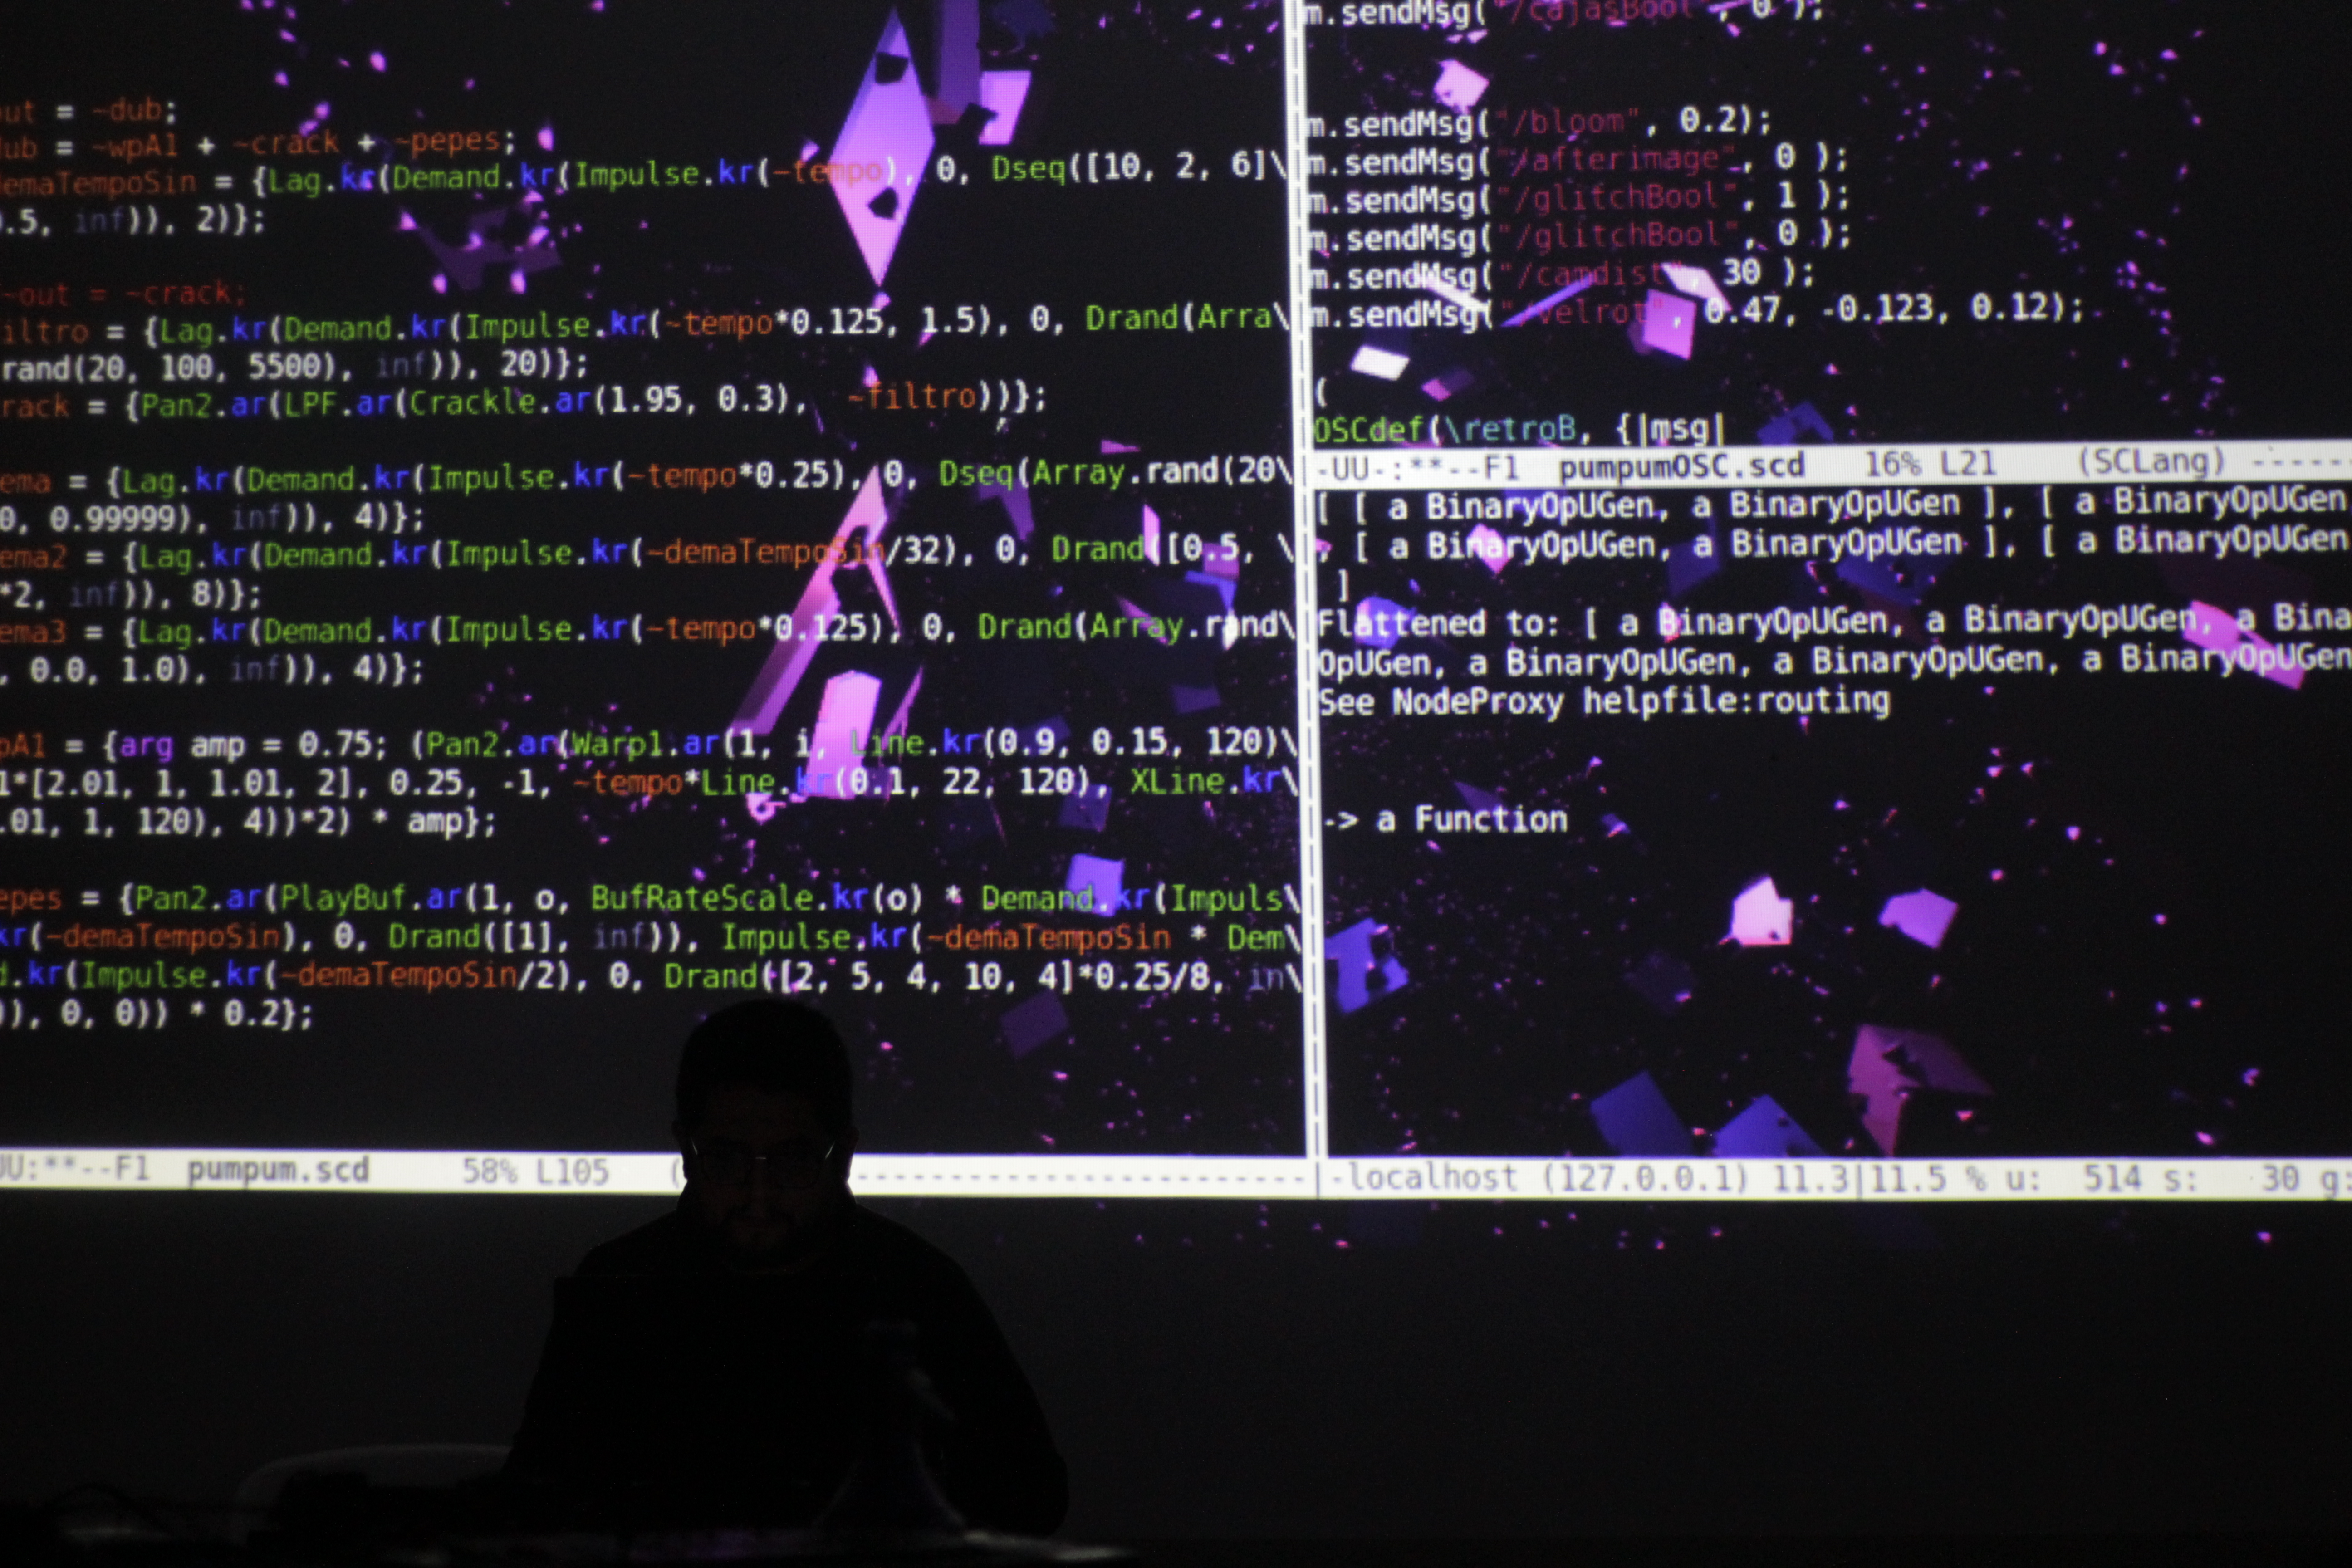
\includegraphics[width=\columnwidth]{../img/pumpum.JPG} 
%\caption[Concierto PUMPUM]{Presentación en el festival PUMPUM} % The text in the square bracket is the caption for the list of figures while the text in the curly brackets is the figure caption
%\label{fig:gallery} 
%\end{figure}

%\subsection{Concierto de clausura} % Este si podría ser relevante 

%Concierto virtual realizado en el marco del coloquio de alumnas del Programa de Posgrado en Música de la UNAM

%\begin{figure}[tb]
%\centering 
%\includegraphics[width=\columnwidth]{../img/col2.png} 
%\caption[Concierto coloquio]{Captura del concierto del Coloquio de alumnas \url{https://youtu.be/HwBTRQKr9Ps}.} % The text in the square bracket is the caption for the list of figures while the text in the curly brackets is the figure caption
%\label{fig:gallery} 
%\end{figure}

\section{PiranhaLab}

Otro antecedente de este proyecto es la práctica y reflexión planteada en colectivo por\textit{PiranhaLab}\footnote{``PiranhaLab es un laboratorio interdisciplinario que trabaja en las tripas del software''. \url{https://piranhalab.github.io/} (Consultado el \today)}.

%\subsection{Escritura de y con software}

%\subsection{Ciclo de Talleres}

El ciclo de talleres realizado en el Centro de Cultura Digital (CCD) en coparticipación con el Laboratorio de Tecnologías Libres\footnote{Actualmente Laboratorio de Tecnologías Compartidas} permitió plantear dos conclusiones que se heredan a \textit{Tres Estudios Abiertos}: La difuminación de la distinción usuario/desarrollador como una motivación para la escritura de software y la procuración de diversidad en la escritura de software en América Latina.

%\end{multicols}
%\vspace*{\fill}
\begin{figure} 
\includegraphics[width=\columnwidth]{../img/conversatorio.jpg} 
\caption[Conversatorio CCD]{Conversatorio organizado por PiranhaLab y el Laboratorio de Tecnologías Compartidas en el CCD. 2019.} % The text in the square bracket is the caption for the list of figures while the text in the curly brackets is the figure caption
\label{fig:gallery} 
\end{figure}
%\clearpage
%\begin{multicols}{1}
  %\raggedright
  
%\subsection{EDGES 2020}

La escritura de espacios para el ciclo de conciertos EDGES 2020 realizado por el Taller de Imágenes en Movimiento del Centro Multimedia (CMM) permitió la exploración de entornos tridimensionales inmersivos en el navegador en el contexto del encierro causado por la pandemia de COVID-19. Técnica y conceptualmente la escritura de estos espacios digitales influye en el presente proyecto. El artículo \textit{Panorama} \citep{panoramaArticulo} hace referencia de manera extensa al ecosistema de espacios y propuestas que también inciden en \textit{Tres Estudios Abiertos}.

% Esto se articula con las actividades colectivas de la sección casos 

Espacios inmersivos que estuvieron activos de manera simultánea. 

\section{Seminario Permanente de Tecnología Musical} 

El Seminario Permanente de Tecnología Musical (SPTM) es un espacio que se enmarca en el Posgrado en Música, específicamente en la línea de tecnología musical. Parte de las reflexiones de este proyecto de investigación se han abordado ahí y definitivamente se relacionan con investigaciones terminadas o en curso. La participación en este seminario permitió vislumbrar el mapa de investigaciones que se realizan en el Posgrado en Música de la UNAM y en específico, las posibles líneas de investigación que también forman parte del contexo en el que se inscribe esta investigación.

%\subsection{Transferencias Aurales}

Una de las primeras actividades que se realizaron en el marco de este seminario fue el Encuentro Latinoamericano de Música y Tecnología \textit{Transferencias Aurales} que tuvo lugar del 8 al 12 de noviembre de 2021.

%\subsection{Panorama} 

El ciclo de conciertos EDGES 2020 abrió posibilidades de reflexión a partir de la escritura de programas. Estas reflexiones fueron puestas a discusión en un espacio que consolidó una serie de artículos que conforman el libro \textit{Algoritmos Arruinados}. 

%\end{multicols}
%\vspace*{\fill}
\begin{figure} 
\includegraphics[width=\columnwidth]{../img/figura7.png} 
\caption[Distopía - Edges 2020]{Espacio diseñado para Distopía. ZGAMU (Música), LVSTVCVR(visuales e imágenes) y PiranhaLab (Diseño de espacio 3d)} % The text in the square bracket is the caption for the list of figures while the text in the curly brackets is the figure caption
\label{fig:gallery} 
\end{figure}
%\clearpage
%\begin{multicols}{1}
  %\raggedright
  
%\subsection{Semestre 2023-I}

% El trabajo con código ha sido preponderante. 

% \printendnotes



% Tal vez mencionar una descripción más extensa del resumen de cada capítulo. Mientras tanto puede quedar así 

\chapter{Marcos de trabajo}

% Este apartado se parece a una sección de los antecedentes. Creo que podría mover algo de eso por acá para hacer el repaso histórico de las herramientas 
% En este apartado se puede abordar la contradicción tecnológica 

% Antes este apartado se llamaba música algorítmica, supongo que quise retomar las discusiones sobre el uso amplio de estas plataformas es decir, fuera de supercollider

% Ejes fundamentales: programación eficiente y optimizada y otras búsquedas estéticas detrás del código.

% Encuentros en marcos restrictivos: restricción y ofrecimiento 

Este apartado hace referencias a reflexiones que resultaron del trabajo con marcos en la realización de piezas audiovisuales para el navegador. Cuando hablo de marcos me refiero a \gls{altonivel} como SuperCollider, OpenFrameworks, Three.js, Web Audio API entre otros. Si bien el caso de SuperCollider es particular, ya que es motor de audio, lenguaje de progrmación e intérprete al mismo tiempo, considero que marcos como los antes mencionados, guardan una relación abstracta con los motores que los posibilitan ( WebGL, OpenGL e incluso el servidor de SuperCollider como módulo independiente). Esto quiere decir que hay funciones sintetizadas que resuelven problemas específicos que no requieren una reconstrucción de bajo nivel. Dos ejes establecen el flujo de este capítulo:

\begin{itemize}

\item Las intenciones expresivas de programas escritos con lenguajes de programación y la contraposición entre la programación eficiente y optimizada y otro tipo de búsquedas como la ofuscación o el error.

\item El papel que juega la relación restricción y ofrecimiento como conceptos de la interacción humano-máquina (HCI), en la experienciación de los marcos de trabajo y la extensión a partir de funcionalidades básicas. 
  
\end{itemize}

% De manera paralela, se aborda el legado que hila el pensamiento musical algorítmico con las posibilidades de escribir módulos personalizados que permitan extender las posibilidades de motores y plataformas que ya existen y de esta forma, dar un giro personalizado a la expresividad del trabajo con audio e imagen. 

A continuación, relacionamos estos dos ejes con algunas descripciones técnicas de las piezas realizadas en conjunto con esta investigación, al mismo tiempo que las vinculamos con algunos de los marcos que se utilizaron en los distintos momentos de cada pieza.


%\end{multicols}
%\vspace*{\fill}
\begin{figure} 
\includegraphics[width=\columnwidth]{../img/of13.png} 
\caption[Openframeworks 1]{Captura de render realizado con OpenFrameworks} % The text in the square bracket is the caption for the list of figures while the text in the curly brackets is the figure caption
\label{fig:gallery} 
\end{figure}

\clearpage
%\begin{multicols}{2}
  %\raggedright


%%%%%% Nombre pegador relacionado con alguna premisa de la descripción
%%%%%% 

%%%%%%%%%%%%%%%%%%%%%%%%%%%%%%%%%%%%%%%%%%%%%%%%%%%%%%%%%%%%%%%%
%%%%%%%%%%%%%%%%%%%%%%%%%%%%%%%%%%%%%%%%%%%%%%%%%%%%%%%%%%%%%%%%
%%%%%%%%%%%%%%%%%%%%%%%%%%%%%%%%%%%%%%%%%%%%%%%%%%%%%%%%%%%%%%%%

\section{La ofuscación como motivo}

Anti es una pieza que surgió como respuesta a tecnologías vinculadas con redes sociales como Instagram o Facebook. En específico, atiende a las tecnologías que permiten el diseño de experiencias, capas y filtros en Realidad Aumentada. En un conjunto de herramientas como la que ofrece Meta Spark ( antes llamado Spark AR), la personalización de las capas que se superponen a una imagen fija o en movimiento está determinada por una interfaz que acota las posibilidades de estas tecnologías al mismo tiempo que facilita su uso.

%\end{multicols}
%\vspace*{\fill}
\begin{Figure}
\includegraphics[width=\columnwidth]{../img/antiHydra1.png}
\captionof{figure}[Anti portada]{Portada del primer momento de Anti. La versión actual se puede consultar en: \url{https://anti.ocelotl.cc}.} % The text in the square bracket is the caption for the list of figures while the text in the curly brackets is the figure caption
\label{fig:gallery} 
\end{Figure}
%\clearpage
%\begin{multicols}{2}
  %\raggedright

Para la realización de Anti, tomé una decisión inicial que contemplaba tres caminos: el uso de Meta Spark, \Gls{openframeworks} o algún tipo de instancia para la web basada en P5.js o \Gls{threejs}.

Como parte del conjunto de restricciones que formaron parte de la intención inicial de este proyecto, Meta Spark quedó desacartada por ser una herramienta privativa. El uso de herramientas de software libre o código abierto puede ser muy ambiguo si consideramos que las licencias que sustentan estos estatutos tienen variaciones que por un lado pueden reforzar visiones optimistas pero poco efectivas en el campo profsional y que por otro, se adscriben a modelos que apoyan a proyectos o instancias con poca claridad en el manejo de datos como Facebook. Sin embargo, como parte de las decisiones subjetivas de este proyecto, considero que hay una frontera fundamental que se relaciona con una intención política pero también con una implicación de accesibilidad: experiencias que solamente pueden ser accedidas por medio de una red social, plataformas de creación de capas tipo filtro que solamente funcionan en un sistema operativo e incluso, la restricción que implica el uso de tarjetas gráficas dedicadas o cualquier tipo de escalada en los recursos físicos de la computadora o dispositivo desde el cual se accesa.

%\end{multicols}
%\vspace*{\fill}
\begin{Figure}
\includegraphics[width=\columnwidth]{../img/anti01.png}
\captionof{figure}[Anti]{Anti e interfaz gráfica. \url{https://anti.ocelotl.cc}.} % The text in the square bracket is the caption for the list of figures while the text in the curly brackets is the figure caption
\label{fig:gallery} 
\end{Figure}
%\clearpage
%\begin{multicols}{2}
  %\raggedright

  La premisa principal de Anti fue la exploración en términos visuales y sonoros del concepto ofuscación audiovisual de voz y rostro. El objetivo de la premisa tecnológica fue intervenir de alguna manera la cara que es capturada por una cámara y el audio que es registrado por un micrófono. Del lado del audio, no se utilizó algún tipo de análisis para transformar la voz, bastó con un filtro de granulación que permitiera modificar la voz sin que esta pudiera ser reconocible pero que pudiera seguir transmitiendo palabras entendibles por un escucha externo. Del lado de la imagen implementé un modelo de TensorFlow previamente entrenado de reconocimiento de puntos clave del rostro\footnote{El modelo específico que utilicé fue face-landmarks-detection. La colección de modelos se encuentra en: \url{https://github.com/tensorflow/tfjs-models}. Consultado el \today}. Hay tres ventajas de este modelo sobre de otros: la información no pasa por servidor externo, el modelo no busca detectar y diferenciar rostros y el nivel de precisión del modelo es bastante alto\citep{kartynnik2019realtime}.

  Como el modelo se ejecuta en Javascript, fue posible incorporarlo de una manera nativa a las librerías de renderado tridimensional y de audio. Eso generó un sistema relativamente eficiente e integrado que si bien no explora la ofuscación en términos del código mismo, si busca tener una intención en términos de la configuración de una herramienta tecnológica con un objetivo cotidiano como es ofuscar la información que se puede extraer del rostro y de la voz, sobre términos de la identificación, seguimiento y vigilancia del individuo. La ofuscación como motivo desdibuja la identidad para conservarla en un anonimato que puede ser compartido y que puede ser el prinicipio de otras formas de pensar la relación el humano como agente y el código como una tecnología imputada de un sentido que no solamente persigue la eficiencia.  

%\end{multicols}
\vspace*{\fill}
\begin{figure}
\includegraphics[width=\columnwidth]{../img/felicidades.png}
\captionof{figure}[Foto de perfil]{Captura de la primera imagen de Anti subida a Google como foto de perfil en la que no se reconoce el rostro.} % The text in the square bracket is the caption for the list of figures while the text in the curly brackets is the figure caption
\label{fig:gallery} 
\end{figure}
%\clearpage
%\begin{multicols}{2}
%\raggedright
  
Precisando en la discusión, la ofuscación puede definirse como el acto deliberado de encubrir el significado de una comunicación. Para el caso de la programación y apuntando ideas hacia los estudios del software, la presente investigación toma la noción de ofuscación de un conjunto de posibilidades para la escritura de software que coinciden, dialogan o se enfrentan a que podríamos definir como la convención de la \emph{estética del código} y aquellos programas que exploran ``otros principios estéticos'' además de los convencionales.

Edsger Dijkstra conoincide con la delimitación convencional de esta forma de escribir programas:

\begin{quote}
``[..] el programador no difiere de algún otro artesano: a menos de que ame sus herramientas, es altamente improbable que pueda crear algo de calidad superior. Al mismo tiempo estas consideraciones nos hablan de las más grandes virtudes que un programa puede mostrar: Elegancia y Belleza''\citep[p.~10]{EWD:EWD35}
\end{quote}

Como respuesta a la posición de Dijkstra y en un ámbito de programación que se aproxima lúdicamente a la escritura de programas, la ofuscación:

\begin{quote}
`` arroja luz a la naturaleza del código fuente, que es leído por un humano e interpretado por una máquina, y puede recordar a los críticos la búsqueda por diferentes dimensiones de sentido y múltiples codeos en todo tipo de programas''\citep[p.~198]{obfuscatedCode}
\end{quote}

El código su lectura, así como las funciones de los programas que ejecuta, son subjetivas y están determinadas por un sentido imputado que socialmente se acuerda de manera tácita y que puede ser visibilizado para interpelarlo en un sentido crítico, lúdico e incluso satírico.\footnote{Tal es el caso de Windows 93 del artista Jankenpopp. \url{https://www.windows93.net/} } En este punto encontramos conexiones con las posibilidades de la programación en una dimensión artística:

\begin{quote}
``[La práctica de la programación ofuscada] sugiere que el codeo puede resistir a la claridad y a la elegancia para pugnar en su lugar por la complejidad, puede hacer familiar lo desconocido y puede luchar con el lenguaje en el que está escrito, justo como lo hace la literatura contemporánea.''\citep[p.~198]{obfuscatedCode}
\end{quote}

La ofuscación puede definirse como el acto deliberado de encubrir el significado de una comunicación. Para el caso de la programación y apuntando ideas hacia los estudios del software, la presente investigación toma la noción de ofuscación de un conjunto de posibilidades para la escritura de software que coinciden, dialogan o se enfrentan a que podríamos definir como la convención de la \emph{estética del código} \citep{EWD:EWD35} y aquellos programas que exploran ``otros principios estéticos'' \citep{obfuscatedCode} además de los convencionales.

¿Puede el código fuente ``luchar'' en contra del marco de uso para el que fue escrito?

    
\section{Tres Estudios}

La práctica artística en contextos audiovisuales y performáticos que realicé hasta 2020 estuvo asociada al uso de SuperCollider para el audio y OpenFrameworks para el video. Las primeras aproximaciones a esta relación tecnológica se debió al trabajo realizado con Celeste Betancur, Jessica Rodríguez, Iracema de Andrade y Alejandro Brianza. Altamisa y Leviatán fueron dos piezas que implementaron esta relación y con apoyo de Celeste Betancur, fue posible realizar un sistema que pudiera detonar videos de acuerdo a decisiones que fueron controladas por medio del protocolo OSC. Esta relación fue ampliamente explorada y en particular, las relaciones y la composición centrada ya no únicamente en audio o video sino en flujos compartidos de información. Este eje continúa presente en la actualidad.

El tránsito de la relación SC y OF hacia Javascript fue motivado por las exigencias tecnológicas que implicó la transmisión de audio e imagen para espacios virtuales. El dominio tecnológico de una nueva herramienta puede suponer un reto y una curva de aprendizaje que requiere dedicación de tiempo. Consideramos que estas curvas pueden reducirse si en el proceso de escritura de código hay información sobre los antecedentes históricos y las ideas que conducen el funcionamiento fundamental de los marcos de trabajo. En este sentido, podemos realizar una observación comparativa entre la plataforma anteriormente utilizada (OF) y Three.js.

%\end{multicols}
%\vspace*{\fill}
\begin{figure}
\includegraphics[width=\columnwidth]{../img/imagen2.png}
\captionof{figure}[THREE.studies]{Captura de la primera versión de THREE.studies} % The text in the square bracket is the caption for the list of figures while the text in the curly brackets is the figure caption
\label{fig:gallery} 
\end{figure}
\clearpage
%\begin{multicols}{2}

OpenFrameworks tiene una forma de concebir el espacio tridimensional, los objetos y las texturas de manera muy similar a Processing en tanto que son objetos que pueden ser invocados y se envuelven entre sí. Para el caso de Three.js, la aproximación se parece mucho más a la forma con la que se conciben los espacios y objetos tridimensionales en programas de diseño y modelado en tres dimensiones. En este sentido es posible trabajar de manera independiente con geometrías, materiales y mallas. 

Comparativa entre OpenFrameworks y Three.js. Estándares del trabajo con imagen que se heredan a través de Processing y que vienen de ideas más antiguas. 

El verdadero reto está en coinciliar los tiempos del audio y el video, siendo que cada uno corre en distintas tasas.

\section{La investigación compilada}

Como se mencionó en la introducción de esta investigación, este texto busca tener dos tipos de salidas: la primera es el texto fijado, impreso o en PDF y la segunda, una serie de recursos que giran en torno al texto y que pueden ser compiladas para el navegador web. 

\begin{comment}
El capitulo toma en consideración el estado actual de la relación entre música y lenguajes de programación como producto de una serie de ideas y perspectivas que han sido heredadas desde plataformas como Music N\citep{cambridgeElectronic} que derivan en interfaces delimitadas que interactúan con motores como SuperCollider o Chuck como Tidal Cycles\citep{mcleanTidal}

el rastreo histórico sobre la relación entre música y lenguajes de programación
Plataformas como Music N y el rastreo que hace Ge Wang sobre este tema.

\section{Legado Audio}

\subsection{Marcos de audio}

A continuación, haremos un breve rastreo de ideas centrales en la escritura de software orientado a la creación musical. El objetivo de este apartado consiste en describir y detectar la presencia del concepto unidad generadora en diversos programas orientados a la generación musical, de entre los cuales está una de las librerías que la presente investigación implementa.

El punto de partida de esta indagación es MUSIC N, proyecto de Max Mathews que sería el parteaguas del paradigma de la música por computadora. Uno de los primeros casos de esta instancia es el principio de programas como Max/MSP y PureData, proyectos representativos de la programación gráfica presente en flujos de trabajo gráfico actuales como TouchDesigner.

Como una observación adicional, es importante detectar instancias de la programación gráfica y de las ideas principales de la música por computadora en plataformas con giros programáticos particulares. Tal es el caso de OpenMusic, que de manera específica está basado en Common Lisp.

Desde la perspectiva de la programación escrita, destacamos el papel que ha tenido SuperCollider en la extensión del paradigma de la música por computadora en la actualidad. Señalamos la importancia de SuperCollider como el motor bajo el cual se pueden ejecutar entornos de programación al vuelo como Tidal Cycles o FoxDot. 

Estuary es un caso adicional que permite establecer un puente entre Tidal Cycles como un entorno que ejecuta SuperCollider como motor de audio y el navegador como tecnología multiplataforma sin instalaciones. Esta plataforma utiliza secuenciadores basados en la sintaxis de Tidal Cycles pero a diferencia del entorno que se puede instalar de manera local en una computadora, Estuary utiliza al navegador como motor de audio. 

Trazamos estas relaciones para establecer una relación continua y presente entre los entornos anteriormente descritos y una de las librerías utilizadas en los casos de estudio de esta investigación: Tone.js. En este sentido, consideramos importante la adscripción a los principios de la música por computadora para encontrar soluciones personalizadas para el navegador.


\subsection{Jacktrip y la música conectada}

Una parte de los antecdentes de este proyecto se vinculan con la actividad del colectivo RGGTRN\footnote{\url{https://rggtrn.github.io/}. Consultado el \today} y del LiveCodeNet Ensamble\footnote{\url{https://livecodenetensamble.wordpress.com/}. Consultado el \today}

RGGTRN es un colectivo de música por computadora fundado por Luis N. Del Angel y Emilio Ocelotl. Posteriormente se unieron Marianne Teixido y Jessica A. Rodríguez. Como parte de un ejercicio lúdico y de reflexión, el colectivo explora la improvisación audiovisual realizada por medio de código de programación, con una relación al contexto Latinx de sus participantes.

% Tesis de Luis
% Bellacode
% Saborítmico
% Tesis de maestría de hernani
% Artículo de Hernani en algún lado
% Artículos de Jessica ? 

raspis conectadas y jacktrip > el trabajo realizado por CCRMA y en general 

La labor del colectivo Radiador

% La radio y la transmisión de sonido con Icecast 

Sonobus y la resolución de problemas de streaming en tiempos de pandemia

\begin{itemize}
\item SuperCollider
\item CommonMusic 
\item Incluso plataformas de más alto nivel de lo que se trata en esta investigación como Megra, Tidal Cycles, Maximilian, Punctual o Conduct.
\item Max/MSP
\item WebAudioAPI
\item ¿DAWs? 
\end{itemize}

\section{Legado Video}

\subsection{Fluxus y openGL}

Para el caso de la imagen, retomo la influencia que tiene en la comunidad de live coding y en mi experienciación del performance audiovisual con la computadora el papel que tuvo el desarrollo Fluxus\footnote{\url{https://gitlab.com/nebogeo/fluxus/}} de Dave Griffiths que se remonta al 2007. Una característica peculiar de este desarrollo es el uso de una sintaxis tipo LISP que recuerda a desarrollos musicales basados en este lenguaje de programación como OpenMusic. 

Detrás de Fluxus también cabe destacar la importancia de sistemas de renderización de gráficos por computadora como OpenGL, que actualmente, son el punto de partida de software de alto nivel involucrado con este proyecto como OpenFrameworks y la variante para el navegador, webGL, que implementa la librería Three.js 

% Pregunta, esto no tendría que ir en otros momentos? Tal vez disperso o tal vez en la introducción 


\begin{itemize}
\item OpenFrameworks 
\item TouchDesigner y plataformas como 
\item Processing
\item Hydra
\item Three.js 
\end{itemize}

\section{El navegador como entorno intergrado} % Este apartado antes se llamada AV / Javascript

% Experiencia de Notas de Ausencia y de Panorama % Esto queda comentado, ya aparece en el apartado de antecedentes 

El anterior repaso da cuenta de los programas y plataformas que anteceden a esta investigación. Están enmarcadas en aplicaciones que se ejecutan localmente y que en ciertos casos, dependen directamente del sistema operativo en el que se ejecutan. A continuación, hablaremos del rumbo que tomó esta investigación hacia el navegador. Sobre este aspecto, destactamos dos resultados que articulan esta decisión:

\begin{itemize}
\item Estructuras compartidas fuera de un marco de trabajo como los que se han enunciado hasta el momento. Esto quiere decir que el navegador y el trabajo específico con Javascript permite organizar los motores gráficos y de audio en una estructura sin que esto requiera de algún tipo de protocolo de comunicación entre aplicaciones como OSC o MIDI.
\item Aplicaciones que corren en el navegador y que por este motivo, pueden ejecutarse prácticamente en cualquier sistema operativo con un navegador. Esto incluye a sistemas operativos para dispositivos móviles como iOS o Android. El coste de recursos es una limitación y la ausencia de un proceso de instalación podría ser una ventaja. % Revisar si esto ya está dicho 
\end{itemize}

% \section{Sistemas operativos y el navegador} % Estos dos módulos se pueden fundir, ojo con que no se descompensen los problemas
% No estoy muy seguro si aquí se pueden escribir las ideas de las secciones anteriores. Podría funcionar la reflexión sobre linux en esta parte? 
% EL papel que juegan las diferencias entre sistemas operativos, las aplicaciones multiplataforma. El navegador es una resolución a estas diferencias pero con un costo alto. % Esto ya estaba antes 
% El navegador como un sistema operativo entre sí (idea de Niklas Reppel). 

%%% Esto ya esta visible otra vez, quitar para la versión estable 

  La ofuscación puede definirse como el acto deliberado de encubrir el significado de una comunicación. Para el caso de la programación y apuntando ideas hacia los estudios del software, la presente investigación toma la noción de ofuscación de un conjunto de posibilidades para la escritura de software que coinciden, dialogan o se enfrentan a que podríamos definir como la convención de la \emph{estética del código} y aquellos programas que exploran ``otros principios estéticos'' además de los convencionales.

Edsger Dijkstra conoincide con la delimitación convencional de esta forma de escribir programas:

\begin{quote}
``[..] el programador no difiere de algún otro artesano: a menos de que ame sus herramientas, es altamente improbable que pueda crear algo de calidad superior. Al mismo tiempo estas consideraciones nos hablan de las más grandes virtudes que un programa puede mostrar: Elegancia y Belleza''\citep[p.~10]{EWD:EWD35}
\end{quote}

Como respuesta a la posición de Dijkstra y en un ámbito de programación que se aproxima lúdicamente a la escritura de programas, la ofuscación:

\begin{quote}
`` arroja luz a la naturaleza del código fuente, que es leído por un humano e interpretado por una máquina, y puede recordar a los críticos la búsqueda por diferentes dimensiones de sentido y múltiples codeos en todo tipo de programas''\citep[p.~198]{obfuscatedCode}
\end{quote}

El código su lectura, así como las funciones de los programas que ejecuta, son subjetivas y están determinadas por un sentido imputado que socialmente se acuerda de manera tácita y que puede ser visibilizado para interpelarlo en un sentido crítico, lúdico e incluso satírico.\footnote{Tal es el caso de Windows 93 del artista Jankenpopp. \url{https://www.windows93.net/} } En este punto encontramos conexiones con las posibilidades de la programación en una dimensión artística:

\begin{quote}
``[La práctica de la programación ofuscada] sugiere que el codeo puede resistir a la claridad y a la elegancia para pugnar en su lugar por la complejidad, puede hacer familiar lo desconocido y puede luchar con el lenguaje en el que está escrito, justo como lo hace la literatura contemporánea.''\citep[p.~198]{obfuscatedCode}
\end{quote}

La ofuscación puede definirse como el acto deliberado de encubrir el significado de una comunicación. Para el caso de la programación y apuntando ideas hacia los estudios del software, la presente investigación toma la noción de ofuscación de un conjunto de posibilidades para la escritura de software que coinciden, dialogan o se enfrentan a que podríamos definir como la convención de la \emph{estética del código} \citep{EWD:EWD35} y aquellos programas que exploran ``otros principios estéticos'' \citep{obfuscatedCode} además de los convencionales.

¿Puede el código fuente ``luchar'' en contra del marco de uso para el que fue escrito?

% Para la versión expandida podría citar las referencias 
% En este punto puedo retomar las ideas de djisktra y de knuth 

Esta definición es el punto de partida de \emph{Anti}, una pieza audiovisual para el navegador que tiene dos objetivos: visibilizar la discusión en torno a el uso de datos y la responsabilidad tecnológica del usuario y 2) actuar como un dispositivo de ofuscación facial y vocal que pueda utilizarse en situaciones de uso cotidiano. 

El maquillaje y el uso de accesorios anti-vigilancia son estrategias analógicas para evitar la detección de rostros. En una situación de protección fuera del entorno digital, incluso una máscara de leds puede cumplir esta función.

El presente proyecto se enfoca los mecanismos de anti-vigilancia que pueden realizarse de manera digital, teniendo a la computadora como un agente intermedio entre dos puntos que desean mantener algún tipo de comunicación gestual y vocal sin que estos puedan detectarse o asociarse a sujetos específicos, sin que esto implique que la comunicación sea completamente ofuscada para los usuarios.
\end{comment}
 % programación eficiente y optimizada vs otras búsquedas estéticas 
\chapter{Expresividad}

% Aquí podría ir la parte de live coding 

\section{Live Coding} % Pregunta: Este apartatdo no debería ir antes ? En momentos anteriores menciono la cuestión  

% Antecedentes más extensos

Encuentro múltiples formas de abordar el tema. El live coding puede describirse en térrminos de unaa comunidad que realiza una práctica y que se enuncia como tal, como un sub-campo creativo que comparte elementos con otra expresiones como la música algorítmica y el arte generativo. Finalmente, el live coding podría acotarse a motivos de investigación académica e independiente y a la realización tecnlógica de interfaces de texto que corren sobre motores de audio y video.

De estas múltiples formas de abordar el fenómeno y de acuerdo a los fines de esta investigación, nos preguntamos si el eje que las articula son discusiones sobre el lenguaje y la escritura. 

\subsection{Primeras expresiones}

Antecedentes del live coding: la escena mod.

En el manifiesto del live coding se expresan pensamientos que hasta el momento, son vigentes. 

% PhD Thesis: Artist-Programmers and Programming Languages for the Arts - Alex McLean 
Dentro de los antecedentes está la experiencia performática de escribir código al vuelo con fines creativos, audiovisuales y experimentales.

Las primeras expresiones reflexivas y prácticas del live coding no solamente establecen puntos de partida performáticas, sino que al mismo tiempo aportan elementos para el diseño y análisis de sistemas basados en interfaces de código:

\begin{quote}

  ``Nuestro argumento nos lleva a través de capas de representación, comenzando con símbolos, luego palabras, lenguaje y notación, para considerar el papel que estas representaciones pueden jugar en la creatividad humana'' \citep[p.~3]{McLean2011}

\end{quote}

La noción de capas de representación permite analizar la complejidad del proceso artístico con código en términos de la relación entre humanos y los aspectos cognitivos, sociales y políticos que les atraviesan, y los no-humanos en lo que respecta a las posibilidades de conocimiento instanciado presentes en ellos. 

Live coding desde cero y la improvisación. 

\subsection{Nodos y circuitos}

La práctica de la programación al vuelo, delimitada técnica, escénica, musical y visualmente se origina en Inglaterra. % cita

Como lo describen \cite{villasenor} para los casos de Barcelona y Ciudad de México.\footnote{Un ejemplo reciente se encuentra en: \url{https://youtu.be/n5kwi4eRAE4}} 

\subsection{Exploración visual}

Exploración visual para la integración con el sonido.  

\begin{figure}[tb]
\centering 
\includegraphics[width=\columnwidth]{../img/of13.png} 
\caption[Openframeworks 1]{Captura de render realizado con OpenFrameworks} % The text in the square bracket is the caption for the list of figures while the text in the curly brackets is the figure caption
\label{fig:gallery} 
\end{figure}

El campo del live coding tuvo un giro importante con la llegada de hydra de Olivia Jack. La rápida expansión de esta plataforma y la sintaxis que recuerda la conexión de flujos de energía similar a los sintetizadores analógicos favorecieron la producción de piezas e interpretaciones enfocadas en la imagen y en algunos otros casos a la par del audio. La importancia de esta plataforma ha delimitado una estética  basada en  la transformación de píxeles, de formas y de transformaciones basadas en funciones matemáticas.

En palabras de Olivia Jack, los procesos que realiza la computadora hay un eje de profundidad, en términos del despliegue gráfico físico de la computadora de espacios bi o tridimensionales, el resultado es bidimensional.

La lógica de Hydra es modular, esto quiere decir que puede incorporarse como un componente adicional a proyectos que no necesariamente se centren en la producción visual con esta plataforma. Esta modularidad juega a favor de lenguajes de programación como Javascript. 


\section{Modo estático}

Piezas fijas y la composición conducida por (bases) de datos 
Sonificación-Visualización
La tradición electroacústica-acusmática 

\section{Modo dinámico}

Live coding y captura gestual 
El problema de la expresividad con algo que aparentemente no es gestual 

\section{Intermedio}

Esas estructuras pueden ser fijas o dinámicas y dependen de varios niveles de profundidad que las significan y las ejecutan
En la práctica, cualquier entorno está en esta mediación. Trabajo muerto acumulado anteriormente. Reflexionar sobre esto
 % Programación fija y programación dinámica 
\chapter{Extensión y escritura}

En este capítulo hablaremos de dos aspectos que detonan reflexión referente a la escritura de módulos de software personalizados.

\begin{itemize}
\item La escritura con lenguajes de programación como una posibilidad para la reconfiguración de las distinciones entre usuarios y desarrolladores.
\item El papel de la diversidad tecnológica en la extensión de los marcos de trabajo y la resistencia a la escalada de recursos computacionales
\end{itemize}

En este sentido, destaco el papel que tiene la extensión de las funcionalidades de marcos de trabajo y lenguajes de programación. En particular, es de interés de este trabajo destacar la ampliación de estas posibilidades de cara a las consecuencias poéticas de piezas construídas con lenguajes de programación. Estas librerías adicionales también pueden perseguir, de manera paralela, objetivos funcionales que pueden medirse de alguna manera. 

\section{Modulos personalizados}

Escritura de bibliotecas para alcanzar una expresividad intermedia.
¿Qué implica escribir módulos personalizados?
Primero que no existan antecedentes y que la idea en lo general pueda al menos realizarse técnicamente.

\section{Reconfiguración de distinciones}

Acción: reconfigurar la distinción usuario/desarrollador-escritor
PLab como casos. Espacio de encuentro y tecnodiversidad
Declaración/acción

\section{Acción e idea}

El código como intepretación y como partitura
Valoraciones del código: elegancia y ofuscación
Encuentros y brechas entre escritura de código, de productos académicos y de algo más abierto.
 % Distinción usuario y desarrollador 
\chapter{Integración} 

Recursividad
Documentos que se ejecutan 

% Quitar esto,  pensar más en un libro de autor
% ¿Cómo convertir tu tesis en un libro?

%\subsection{Resultados}

% Pienso que esto podría sustituirse por integración pero no sé, siento que aquí hay algo redundante

%Como un repaso de lo que está escrito antes, apuntes para las conclusiones
 % La brecha entre las escrituras 
\chapter{Conclusiones}

% Esto sirve como una propuesta para las conclusiones 

%\begin{quote}
%  ``Esta aproximación estética no solamente incluye una introducción a la programación de manera práctica y creativa, sino también el cultivo de un espacio abierto donde sea posible discutir y reflexionar sobre la cultura computacional.''\citep[p.~87]{soonKnotts}
%\end{quote} 

% En procesos de formativos y de reflexión pero también en espacio de investigación como el seminario permanente de tecnología musical 

% La imposibilidad de encontrar un equilibrio entre lo tecnológico, lo poético y lo investigativo 

 % Hacerlo más eficiente es como asumir el acerelacionismo ? 

%\input{../perspectivas/perspectivas}

\addcontentsline{toc}{chapter}{\protect\numberline{}Referencias}%
\bibliography{../bib/panBib}{} 
\bibliographystyle{../bib/apalike-es}
\clearpage

\printglossaries

% \end{multicols}

\end{document}
